\documentclass[11pt]{article}
\usepackage[margin=1in]{geometry}
\usepackage{amsmath,amssymb,amsthm,booktabs,longtable,hyperref}
\usepackage{tikz}
\usetikzlibrary{arrows.meta,positioning}
\newtheorem{theorem}{Theorem}
\newtheorem{lemma}[theorem]{Lemma}
\newtheorem{proposition}[theorem]{Proposition}
\newtheorem{corollary}[theorem]{Corollary}
\theoremstyle{remark}
\newtheorem{remark}[theorem]{Remark}
\newtheorem{example}[theorem]{Example}
\emergencystretch=3em\newcommand{\ML}{\mathrm{ML}}
\newcommand{\R}{\mathbb{R}}
\newcommand{\Z}{\mathbb{Z}}
\newcommand{\Q}{\mathbb{Q}}
\newcommand{\dist}[1]{\lVert #1\rVert}
\newcommand{\lean}[1]{{\small\texttt{\detokenize{#1}}}}
\title{The four-speed lonely runner spectrum below $1/4$:\\ a kernel-checked formalization}
\author{Vico Bonfioli}
\date{November 2026}
\begin{document}
\maketitle

\begin{abstract}
For positive integer speeds $v_1,\dots,v_n$ let $\ML(v)=\max_{t}\min_i\dist{tv_i}$, where $\dist{x}$ is the distance to the nearest integer. Theorem~1.2 of Yi, Gill and Bu~\cite{YGB} states that for four distinct positive integer speeds the values of $\ML$ below $1/4$ are exactly $j/(4j+2)$ with $j\ge2$, $j\ne3$. Their proof is effective and computer assisted (an exact search over $800{,}816{,}099$ quadruples, with ancillary code in C and Python and no proof assistant). Jain and Kravitz~\cite{JK}, Theorem~1.3, had shown the statement up to an ineffective finite set, and Fan and Sun~\cite{FanSun}, Conjecture~4.1, had conjectured it. We give a complete formalization of the statement in Lean~4 with Mathlib: the inclusion, the attainment of every value $j/(4j+2)$ and the equivalence, with no \lean{sorry} and no axiom beyond the three standard ones. The proof uses a computer-assisted certificate (15 depth-one nodes, 5{,}010 child points, 4{,}998 noncritical leaf records, 408{,}232 line checks, 765 kernel-evaluated theorems, each covering a block of leaf records) that the Lean kernel checks, an exact analysis of the two infinite families of speeds on the critical tori, and one sporadic tuple, $(1,3,4,14)$. The theorem is not new; the contribution is the kernel check and the exact tail analysis. To our knowledge, as of searches made on 17 November 2026, no other formal proof of the statement is known.
\end{abstract}

\section{Introduction}\label{sec:intro}

For a vector $v=(v_1,\dots,v_n)$ of positive integers put
\[
\ML(v)=\max_{t\in\R}\ \min_{1\le i\le n}\dist{tv_i},\qquad \dist{x}=\min(\{x\},1-\{x\}).
\]
The lonely runner conjecture asserts $\ML(v)\ge 1/(n+1)$ for $n$ speeds. Kravitz~\cite{Kravitz21} asked which values below $1/n$ occur; for $n=3$ he proved that they are the numbers $s/(3s+1)$. Fan and Sun~\cite{FanSun} found an infinite family showing that the natural analogue fails for $n=4$ (for instance $\ML(8,4r+3,4r+11,4r+19)=(2r+7)/(4(2r+7)+2)$), and conjectured that for four speeds either $\ML\ge1/4$ or $\ML=s/(4s+k)$ with $k\in\{1,2\}$ (their Conjecture~4.1). Jain and Kravitz~\cite{JK} work with $D=\tfrac12-\ML$, so that $\ML<1/4$ means $D>1/4$. Their Theorem~1.3 says that the set of values of $D$ in $(1/4,1/2]$ that occur for four speeds ($S_1(4)$ in their notation) differs from $\{1/4+1/(8s+12):s\ge0\}$ by a finite set that they did not determine. In terms of $\ML$ that progression is $\{j/(4j+2):j\ge1\}$ (put $j=s+1$), and the spectrum proved below omits exactly $j=1$ and $j=3$. Yi, Gill and Bu~\cite{YGB} then proved the full statement: their Theorem~1.2 is exactly Theorems~\ref{thm:main} and~\ref{thm:attained} below, and their Theorem~1.1 classifies the primitive quadruples with $\ML<1/4$. Their proof is effective and computer assisted (an exact search over $800{,}816{,}099$ quadruples; the ancillary package is in C and Python) and uses no proof assistant.

\paragraph{What this paper claims.} We claim exactly one thing: a complete, kernel-checked Lean~4 formalization of the following statement, together with the certificate and the exact tail analysis that the formalization needs. Here complete means that the inclusion (Theorem~\ref{thm:main}), the attainment of every value (Theorem~\ref{thm:attained}) and the equivalence (Corollary~\ref{cor:iff}) are all stated and proved in Lean. We do not claim a first proof of the theorem. The mathematical statement is due to Yi, Gill and Bu~\cite[Theorem~1.2]{YGB}; the proof strategy below (a tree of lattice flags, two critical tori, one sporadic tuple) follows the same overall shape as their classification in Theorem~1.1 of~\cite{YGB}, and our route to the finite part, a flag tree checked in the kernel, is different from their exhaustive search of $800{,}816{,}099$ primitive quadruples. To our knowledge, as of the searches of 17 November 2026 described in Section~\ref{sec:prior}, no other formal proof of the statement is known; Oliner~\cite{Oliner} has Lean statements for the exact values of two families of four speeds (Section~\ref{sec:prior}), and Chen~\cite{Chen} has formalized the lonely runner conjecture for up to seven runners. The only computer-assisted component of the proof is a certificate that the Lean kernel checks. No human expert has reviewed the formal development; Section~\ref{sec:guarantee} says what the kernel check does and does not guarantee.

\begin{theorem}[Lean: \lean{LRSpectrumFull.L4S5.four_speed_spectrum}]\label{thm:main}
Let $v\in\Z^4$ have positive, pairwise distinct entries and $\ML(v)<1/4$. Then $\ML(v)=j/(4j+2)$ for an integer $j\ge2$ with $j\ne3$.
\end{theorem}
\begin{theorem}[Lean: \lean{four_speed_attained}]\label{thm:attained}
For every integer $j\ge2$, $j\ne3$, there are four distinct positive integers $v$ with $\ML(v)=j/(4j+2)$.
\end{theorem}
\begin{corollary}[Lean: \lean{four_speed_spectrum_iff}]\label{cor:iff}
The set of values $<1/4$ of $\ML$ on four distinct positive integer speeds is $\{j/(4j+2): j\ge2,\ j\ne3\}$.
\end{corollary}

\paragraph{Where the idea is.} A near-tight primitive vector $v$ (one with $\ML(v)<1/4$) is encoded by its relation lattice $\Lambda=\{x\in\Z^4:\langle x,v\rangle=0\}$, of rank three. A reduced basis of $\Lambda$ (a \emph{flag}: a basis $(h_0,h_1,h_2)$ chosen greedily, defined in Section~\ref{sec:tree}) and covering-radius bounds on each stage of it turn ``$\ML(v)<1/4$ for infinitely many $v$'' into a finite tree of choices for the first two basis vectors. Each leaf of the tree is either \emph{critical}, which means that the leaf is a $2$-dimensional subtorus of $(\R/\Z)^4$ on which the maximum loneliness is exactly $1/4$ (the two such subtori were classified by Jain and Kravitz~\cite{JK}; Section~\ref{sec:tree} says what is cited and what is proved here; one of them has the \emph{$B_2$ root pattern} $a,b,a+b,2a+b$, the values of the four positive roots $\alpha,\beta,\alpha+\beta,2\alpha+\beta$ of the root system $B_2$ at a point where the simple roots take the values $a,b$), where $\ML$ is an explicit function of residues modulo $4$, or noncritical, with a finite list of vectors, each shown to have $\ML\ge1/4$ by an explicit \emph{time} (a rational $a/q$ with $\min_i\dist{u_ia/q}\ge1/4$), except for two tuples. The picture in one sentence: a primitive $v$ with $\ML(v)<1/4$ has a lattice of relations that is so well reduced that two basis vectors are pinned down by a finite amount of data; for all but two lattices of lines every point has a lonely time and this bounds $|v|$, and on the two exceptional lattices $\ML$ is computed exactly. The tree is finite but too large to check by hand, so the Lean kernel checks it; Section~\ref{sec:finite} explains why it is finite, with a table of its $15$ depth-one nodes (Table~\ref{tab:nodes}) and a worked leaf (Example~\ref{ex:leaf}).

\paragraph{Scope.} Covered: four pairwise distinct positive integer speeds of any greatest common divisor. Not covered, and not stated in Lean: repeated speeds (these reduce to at most three distinct speeds), zero or negative speeds (a signed form follows from invariance of $\ML$ under sign changes but is not stated), non-integer speeds, any number of speeds other than four, and shifted (phase) versions of the problem. Values of $\ML$ that are at least $1/4$ are not described.

\paragraph{Contents.} Subsection~\ref{sec:notation}, at the end of this section, fixes the notation and lists the terms. Section~\ref{sec:outline} gives the proof at one level of zoom, with its dependency diagram. Section~\ref{sec:tails} proves the exact value of $\ML$ on the two critical families. Section~\ref{sec:tree} explains why the tree is finite, works one leaf by hand, states the lattice lemmas with their proofs, and describes the case tree and the certificate that reduce every near-tight vector to those families or to two residual tuples. Section~\ref{sec:sporadic} treats the sporadic tuple. Section~\ref{sec:trust} lists what must be trusted, Section~\ref{sec:repro} how to rebuild the proof, Section~\ref{sec:prior} the prior art and Section~\ref{sec:prov} the provenance of this work. Appendix~A lists the Lean modules.

\subsection{Notation and vocabulary}\label{sec:notation}

This subsection fixes the symbols that are used for more than one object and lists the terms the paper defines, with the place of definition. It uses only the definition of $\ML$ above and is used by every later section as a reference table. Where a letter has two meanings, the section named in the table decides; the text says which meaning is meant when both occur in one paragraph.

{\small
\begin{longtable}{p{2.9cm}p{7.6cm}p{4.0cm}}
\toprule
symbol & meaning & where\\
\midrule
\endhead
$\dist x$, $f(x)$ & distance of $x$ to $\Z$; $f(x)=\min_i\dist{x_i}$ for $x\in\R^4$ & Sections~\ref{sec:intro}, \ref{sec:tree}\\
$t$ & a real \emph{time}; $\ML(v)=\sup_tf(tv)$. The class vector of Section~\ref{sec:tree} is written $\tau\in\Z^3$ & Sections~\ref{sec:intro}--\ref{sec:tails}, \ref{sec:sporadic}\\
$\tau$ & class of the second row $h_1$ modulo $\Z h_0$, $\tau_i=\langle b_i,h_1\rangle$ & Lemma~\ref{lem:child}(i)\\
$j$ & index of the spectrum, $\ML=j/(4j+2)$, $j\ge2$, $j\ne3$ & everywhere\\
$s$, $r$ & $s$: parameter of $(1,2,3,4s)$, with $\ML=s/(4s+1)$ and $j=2s$; $r$: parameter of the Fan--Sun family $(8,4r+3,4r+11,4r+19)$, with $j=2r+7$. Inside proofs $s,r$ are also used as local names (a coefficient, an odd integer) and then are defined on the spot & Section~\ref{sec:tails}\\
$g$, $v'$, $\sigma$, $\varphi$ & $g$: the gcd factor, $v'=v/g$ the primitive part; $\sigma$: a signed permutation of the coordinates; $\varphi$: the pivot speed of the lower bound for the second family (Section~\ref{sec:tails}); never a gcd & Section~\ref{sec:tails}; Step~1\\
$A,B$ & parameters of $(A,2A,3A,B)$ (first torus), coprime and $\ge1$ & Section~\ref{sec:tails}\\
$a,b$ & parameters of $(a,b,a+b,2a+b)$ (second torus), coprime and $\ge1$; $q_1=a+2b$, $q_2=3a+2b$, $q_4=3a+b$, $K_i=\lfloor q_i/4\rfloor$ (an integer), $\nu_i=q_i-4K_i$ & Section~\ref{sec:tails}\\
$c$, $N$, $\xi,\eta$, $X$ & Section~\ref{sec:tails}: $c$ a real upper bound for $\ML$, $N$ an integer ($N=a\lfloor u\rfloor-(a+b)\lfloor w\rfloor$), $\xi,\eta$ fractional parts, $X=2a+b-2K_4-2$. In the paragraph on the second family $u=(a+b)t$ and $w=at$ are real numbers & Section~\ref{sec:tails} (second family)\\
$m_i$, $\ell$ & multipliers of the pivot table and the B\'ezout integer in the lower bound; $m=|v|^2$ is a different object & Section~\ref{sec:tails} (lower bound)\\
$\Lambda$, $h_0,h_1,h_2$ & lattice of integer relations of $v$ and a greedy flag of it (rows numbered from $0$); $L_k=\Z h_0+\dots+\Z h_{k-1}$ & Section~\ref{sec:terms}\\
$\mu_i$, $G_1,G_2,G_3$ & Gram--Schmidt norms ($i=1,2,3$) and Gram minors, $\mu_1^2=G_1$, $\mu_2^2=G_2/G_1$, $\mu_3^2=G_3/G_2$, $G_3=|v|^2$ & Section~\ref{sec:terms}; indices against Lean: proof of Lemma~\ref{lem:prune}\\
$T(L_k)$, $M(L_k)$ & stage torus and its maximum loneliness (not the integer $N$ of Section~\ref{sec:tails}) & Section~\ref{sec:terms}\\
$k$, $d$ & $k\in\{0,1,2\}$ the stage (rows imposed), $d\in\{1,2,3\}$ the depth (rows chosen) & Section~\ref{sec:terms}\\
$x_k/W_k$, $c_k$, $A_k$, $\varepsilon_k$ & witness point of $T(L_k)$ with integer numerators and common denominator $W_k$, its loneliness $c_k$ ($c_k\ge1/4$), $A_k=4\min_i(\text{distance of }x_{k,i}\text{ to }W_k\Z)-W_k$ and $\varepsilon_k=A_k/W_k=4c_k-1$. The integers $A_1,A_2$ are unrelated to the parameter $A$ of the first torus & Table~\ref{tab:nodes}, Lemma~\ref{lem:child}\\
$b_1,b_2,b_3$, $\mathcal B$ & stored basis of $h_0^\perp\cap\Z^4$ and its Gram matrix (not the parameter $B$ of the first torus); $\mathcal B_{ii}$ its diagonal & Lemma~\ref{lem:child}(i)\\
$\Gamma_2$, $k_0,k_1$ & the rank-two lattice $L_2^\perp\cap\Z^4$ of a leaf and its stored basis (called $K_2$ in the Lean sources; it is not the integer $K_2=\lfloor q_2/4\rfloor$ of Section~\ref{sec:tails}) & Section~\ref{sec:terms}\\
$x$, $(x,z)$, $u$ & $x$ is a point of $\R^4$ (a test point or a witness $x_k/W_k$) except in the phrase ``line $u=xk_0+zk_1$ of a leaf'', where $(x,z)$ are integer coordinates; $u$ is a line of a leaf (or a vector of $\Lambda$ in the proof of Lemma~\ref{lem:prune}), and the real number $(a+b)t$ in the second-family paragraph of Section~\ref{sec:tails} & Section~\ref{sec:tree}\\
$H,R,L,D,p,a,w$ & matrices and coordinates used only inside the proof of Lemma~\ref{lem:prune}; there $a$ is a vector of integers and $w$ a vector of reals (not the parameters of Section~\ref{sec:tails}) & proof of Lemma~\ref{lem:prune}\\
$\lambda$, $e$, $\rho$, $\psi_b$ & local names: a rational coefficient and the nearest integer to it; the radius $\frac12\sqrt{S_k}$; integer functionals dual to $h_0,\dots,h_{d-1}$ & proof of Lemma~\ref{lem:prune}\\
\bottomrule
\end{longtable}
}

\emph{Vocabulary.} Each term is defined where indicated. \emph{Near-tight}: primitive, nonzero entries, $\ML<1/4$ (Lean \lean{NearTight}). \emph{Critical torus}, \emph{$B_2$ root pattern}: the two $2$-dimensional subtori on which the maximum loneliness is exactly $1/4$, one of them the values of the positive roots of $B_2$ (introduction and Section~\ref{sec:tails}; classified in~\cite{JK}). \emph{Flag}, \emph{greedy flag}, \emph{stage torus}, \emph{time}, \emph{window}, \emph{leaf}, \emph{line}, \emph{chunk}, \emph{range theorem}, \emph{chunk module}: Section~\ref{sec:terms}. \emph{Node}: a depth-one record, Lemma~\ref{lem:child}(i) and Table~\ref{tab:nodes}. \emph{Critical leaf}, \emph{noncritical leaf}: Section~\ref{sec:tree}, ``What is asked of $T(L_2)$ at a leaf''. \emph{Funnel}: the successive filters applied to the box of candidate second rows, Section~\ref{sec:tree}. \emph{Certificate}: the generated data of Section~\ref{sec:tree} that the kernel checks. \emph{Kernel-checked}: accepted by the Lean kernel, with the guarantee and its limits stated in Section~\ref{sec:guarantee}.

\section{Outline of the proof}\label{sec:outline}

This section proves nothing by itself: it states Theorems~\ref{thm:main} and~\ref{thm:attained} as five macro-steps, says what each step uses, and points to the section that discharges it. It uses only the statements of Section~\ref{sec:intro}; Sections~\ref{sec:tails}--\ref{sec:sporadic} discharge the steps, and no later section uses this one except as a map.

\paragraph{Map of the argument.} The table lists every step, what it uses, where it is argued, and who can check it. Every step is also checked by the Lean kernel; the last column says whether a human can follow the argument on paper (``text'') or whether the step rests on generated data that only the kernel (and the generator) can reproduce (``kernel only'').
\begin{center}
\small
\begin{tabular}{p{1.9cm}p{4.4cm}p{3.1cm}p{1.7cm}p{3.2cm}}
\toprule
step & content & uses & where & who checks\\
\midrule
1 & reduce to primitive vectors with distinct nonzero absolute entries & invariance of $\ML$ under scaling and signed permutations & Sec.~\ref{sec:tails} (start) & text; kernel\\
2a & two lattice lemmas: pruning (Lemma~\ref{lem:prune}) and child step with leaf window (Lemma~\ref{lem:child}) & Gram--Schmidt, nearest-plane rounding & Sec.~\ref{sec:tree} & text (proved in full); kernel\\
2b & certificate: $15$ nodes, $5{,}010$ leaves, $408{,}232$ lines & Lemmas~\ref{lem:prune},~\ref{lem:child}; generated data & Sec.~\ref{sec:tree} & kernel only; a worked leaf by hand (Example~\ref{ex:leaf})\\
2c & tree completeness: every near-tight vector is on a critical torus or is one of two tuples & 2a, 2b, step 1 & Sec.~\ref{sec:tree} (end) & kernel (assembly is hand-written Lean)\\
3 & exact $\ML$ on the two critical families; values $j/(4j+2)$, $j\ge2$, $j\ne3$ & B\'ezout, case analysis on residues mod $4$ & Sec.~\ref{sec:tails} & text; kernel\\
4 & $\ML(1,3,4,14)=4/17$ & nine closed arcs & Sec.~\ref{sec:sporadic} & text; kernel\\
5 & every $j\ge2$, $j\ne3$ occurs & step 3 & Sec.~\ref{sec:tails} & text; kernel\\
\bottomrule
\end{tabular}
\end{center}
Only step 2b is out of reach of a reader without the generator; Section~\ref{sec:trust} says what the kernel guarantees there and what it does not.

\begin{enumerate}
\item \textbf{Normalization.} Replace $v$ by its primitive part $v'=v/g$ (invariance $\ML(gw)=\ML(v')$), and by sorting and sign changes (invariance under signed permutations). Distinct positive entries remain distinct and positive. This suffices because it reduces the theorem to primitive vectors with nonzero entries and pairwise distinct absolute values. (Lean: \lean{exists_prim}, \lean{nf_ML_smul}, \lean{SPS}. The same invariances, together with a reduction in the Weyl group of $B_2$, bring a vector on a critical torus to the normal forms of Step~3; see the paragraph ``Normal forms'' at the start of Section~\ref{sec:tails}.)
\item \textbf{Tree completeness.} If $v'\in\Z^4$ is primitive, has nonzero entries, pairwise distinct absolute values and $\ML(v')<1/4$, then either $v'$ lies on a critical torus, i.e.\ is a signed permutation of $(A,2A,3A,B)$ or of $(a,b,a+b,2a+b)$ up to a common factor, or $v'$ is a signed permutation of one of the two stored residual tuples $(1,2,3,8)$, $(1,3,4,14)$. Of these, $(1,2,3,8)$ is $(A,2A,3A,B)$ with $A=1$, $B=8$, so it lies on the first torus; it is listed because the finite check returns it as a stored tuple (it has no lonely time), not because it is an extra case; only $(1,3,4,14)$ is on neither torus. This suffices because it leaves two explicit families and one explicit tuple to evaluate. Distinctness of the absolute entries is a hypothesis of this step and is used exactly where the line check skips lines with a repeated absolute entry (Section~\ref{sec:tree}); it is not used by Lemmas~\ref{lem:prune} and~\ref{lem:child}. (Lean: \lean{tree_complete4_real}, no unproved hypothesis: its hypotheses are the near-tightness of the vector and the distinctness of its absolute entries, both in the statement of Step~2 above; Section~\ref{sec:tree}.)
\item \textbf{Critical lines.} On $(A,2A,3A,B)$ with $A,B\ge1$ coprime, $\ML\ge1/4$ unless $A=1$ and $B=4s$, where $\ML(1,2,3,4s)=s/(4s+1)=2s/(4\cdot2s+2)$. On $(a,b,a+b,2a+b)$ with $a,b\ge1$ coprime, $\ML=\max(K_1/q_1,K_2/q_2,K_4/q_4)$ with $q_1=a+2b$, $q_2=3a+2b$, $q_4=3a+b$, $K_i=\lfloor q_i/4\rfloor$. In both cases $\ML<1/4$ forces $\ML=j/(4j+2)$ with $j\ge2$, $j\ne3$. This suffices because it settles every vector produced by Step~2 on a critical torus. (Lean: \lean{U1_spectrum}, \lean{U2_exact}, \lean{U2_spectrum}, \lean{four_tails}; Section~\ref{sec:tails}.)
\item \textbf{Residual tuples.} $\ML(1,2,3,8)=2/9=4/18$ ($j=4$) lies on the first torus and is already covered by Step~3 ($s=2$); it is mentioned for completeness. $\ML(1,3,4,14)=4/17$ ($j=8$) is off both tori and is computed directly. This suffices because these are the only other outcomes of Step~2. (Lean: \lean{U1_exc_exact}, \lean{ML_1_3_4_14}; Section~\ref{sec:sporadic}.)
\item \textbf{Occurrence.} Even $j\ge2$ occurs on $(1,2,3,2j)$ (the vector $(1,2,3,4s)$ with $s=j/2$), odd $j\ge7$ occurs on $(8,4r+3,4r+11,4r+19)$ with $j=2r+7$, and $j=5$ at $(7,1,8,15)$. This suffices for Theorem~\ref{thm:attained}, since the three cases exhaust $j\ge2$, $j\ne3$. (Lean: \lean{four_occurs}, \lean{U2_occurs_odd}; Section~\ref{sec:tails}.)
\end{enumerate}
Steps 3--5 are hand-written mathematics checked by Lean. Step 2 is where the computer enters.

\begin{figure}[ht]
\centering
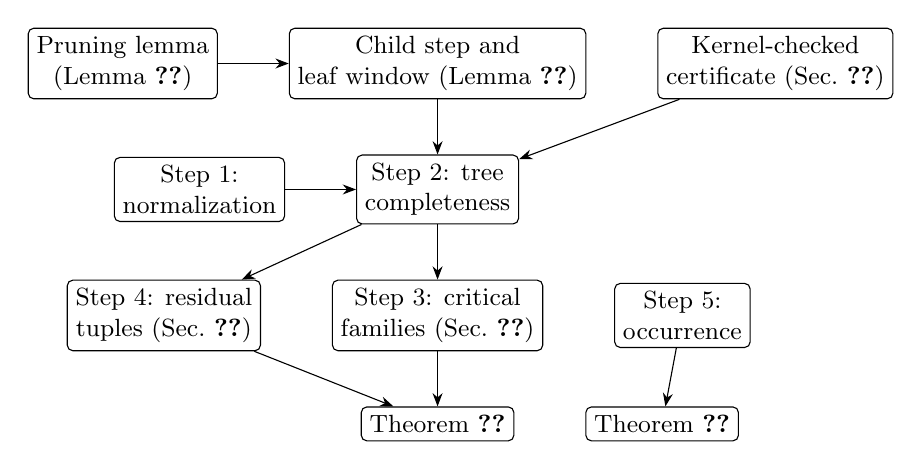
\begin{tikzpicture}[>=Stealth, node distance=7mm and 9mm, box/.style={draw, rounded corners=2pt, align=center, inner sep=3pt, font=\small}]
\node[box] (flag) {Pruning lemma\\(Lemma~\ref{lem:prune})};
\node[box, right=of flag] (child) {Child step and\\leaf window (Lemma~\ref{lem:child})};
\node[box, right=of child] (cert) {Kernel-checked\\certificate (Sec.~\ref{sec:tree})};
\node[box, below=of child] (tree) {Step 2: tree\\completeness};
\node[box, left=of tree] (norm) {Step 1:\\normalization};
\node[box, below=of tree] (crit) {Step 3: critical\\families (Sec.~\ref{sec:tails})};
\node[box, left=of crit] (spor) {Step 4: residual\\tuples (Sec.~\ref{sec:sporadic})};
\node[box, right=of crit] (occ) {Step 5:\\occurrence};
\node[box, below=of crit] (main) {Theorem~\ref{thm:main}};
\node[box, right=of main] (att) {Theorem~\ref{thm:attained}};
\draw[->] (flag) -- (child);
\draw[->] (child) -- (tree);
\draw[->] (cert) -- (tree);
\draw[->] (tree) -- (crit);
\draw[->] (tree) -- (spor);
\draw[->] (norm) -- (tree);
\draw[->] (crit) -- (main);
\draw[->] (spor) -- (main);
\draw[->] (occ) -- (att);
\end{tikzpicture}
\caption{Dependencies of the macro-steps. An arrow from $X$ to $Y$ means that $Y$ uses $X$.}
\label{fig:dag}
\end{figure}

\begin{example}\label{ex:smallest}
We work the smallest case $v=(1,2,3,4)$ by hand, and two further tuples. Here $\ML(1,2,3,4)=1/5=j/(4j+2)$ with $j=2$ (the case $s=1$ of the first family $(1,2,3,4s)$, where $\ML=s/(4s+1)$). \emph{Lower bound:} at $t=1/5$ the four distances are $1/5,2/5,2/5,1/5$, so $\ML\ge1/5$. \emph{Upper bound:} suppose some $t$ has all four distances $>1/5$. Since $\dist{\cdot}$ is even and $1$-periodic we may take $t\in[0,1/2]$, where $\dist t=t$. Then $t>1/5$. For $t\in[0,1/4]$ we have $\dist{2t}=2t$ and for $t\in[1/4,1/2]$ we have $\dist{2t}=1-2t$, so $\dist{2t}>1/5$ gives $1/10<t<2/5$. Hence $t\in(1/5,2/5)$, so $3t\in(3/5,6/5)$ and $\dist{3t}=|3t-1|$, and $\dist{3t}>1/5$ forces $t<4/15$. Then $4t\in(4/5,16/15)$, so $\dist{4t}=|4t-1|<1/5$, a contradiction. Hence $\ML(1,2,3,4)=1/5$.

The vector $(7,1,8,15)$ is $(a,b,a+b,2a+b)$ with $(a,b)=(7,1)$: $q_1=9$, $q_2=23$, $q_4=22$, so $K_1=2$, $K_2=5$, $K_4=5$ and $\ML=\max(2/9,5/23,5/22)=5/22=j/(4j+2)$ with $j=5$. The tuple $(1,3,4,14)$ has the witness $t=7/17$: the distances are $7/17$, $4/17$, $6/17$, $4/17$.
\end{example}

\section{The two critical families}\label{sec:tails}

This section proves the exact value of $\ML$ on the two infinite families of speeds that Section~\ref{sec:tree} isolates (the critical tori), and derives from it that the values below $1/4$ are of the form $j/(4j+2)$ with $j\ge2$, $j\ne3$, together with the occurrence statement of Step~5. It needs only B\'ezout's identity and linear arithmetic over $\R$ and $\Z$, and nothing from Sections~\ref{sec:tree} and~\ref{sec:sporadic}. Section~\ref{sec:tree} uses its conclusions for every leaf that lies on a critical torus, and the proof of Theorem~\ref{thm:main} uses it for Step~3.

\paragraph{Normal forms.} Step~2 delivers a vector $v'$ on a critical torus in the following general sense (Lean: \lean{OnCritTorus}, \lean{SPS}): there are integers $A,B$ (or $a,b$) and a factor $g\ge1$ such that $v'=g\cdot\sigma$ of $(A,2A,3A,B)$ or of $(a,b,a+b,2a+b)$, where $\sigma$ is a signed permutation of the four coordinates. The parameters are arbitrary integers. The two families below are stated for $A,B\ge1$ (resp.\ $a,b\ge1$) coprime, so a reduction is needed. Lean proves it (\lean{normal_form}) from four facts.
\begin{enumerate}
\item $\ML$ is unchanged by permuting the coordinates, by changing the sign of a coordinate (because $\dist{-x}=\dist x$) and by dividing out a common factor (\lean{nf_ML_perm}, \lean{nf_ML_signs}, \lean{nf_ML_smul}).
\item First torus. All entries of $v'$ are nonzero, so $A,B\ne0$; signs are free, so we may take $A,B\ge1$ (\lean{SPS_U1_abs}); dividing by $\gcd(A,B)$ moves that factor into $g$ (\lean{exists_coprime_split}, \lean{SPS_U1_scale}).
\item Second torus. The entries $a,b,a+b,2a+b$ are the values of the four positive roots $\alpha,\beta,\alpha+\beta,2\alpha+\beta$ of $B_2$ ($\alpha$ short, $\beta$ long) at the point where the simple roots take the values $a,b$. The Weyl group of $B_2$ has order $8$ and permutes the roots up to sign, so replacing $(a,b)$ by its image under a Weyl group element gives a signed permutation of the same vector. We need only three elements, written on $(a,b)$: the reflection $s_\alpha:(a,b)\mapsto(-a,\,2a+b)$, the reflection $s_\beta:(a,b)\mapsto(a+b,\,-b)$ and $-1:(a,b)\mapsto(-a,-b)$. On the vector they act as follows: $s_\alpha$ swaps the second and fourth coordinates and changes the sign of the first (the vector becomes $(-a,\,2a+b,\,a+b,\,b)$); $s_\beta$ swaps the first and third coordinates and changes the sign of the second ($(a+b,-b,a,2a+b)$); $-1$ changes all signs (\lean{SPS_U2_s1}, \lean{SPS_U2_s2}, \lean{SPS_U2_neg}). The Weyl group is not used as a theory; Lean proves by a case split on signs that every $(a,b)$ with $a,b,a+b,2a+b\ne0$ is carried to $a',b'\ge1$ (\lean{U2_to_pos}). If $b<0$ apply $-1$, so assume $b>0$. If $a>0$ stop. If $a<0$ and $2a+b>0$ apply $s_\alpha$, giving $(-a,2a+b)$. If $a<0$, $2a+b<0$ and $a+b>0$ apply $s_\alpha$ then $s_\beta$, giving $(a+b,-2a-b)$. If $a<0$, $2a+b<0$ and $a+b<0$ apply $s_\alpha$, $s_\beta$, $s_\alpha$, giving $(-a-b,\,b)$. In every case both entries are positive. This is the statement that every regular point of the plane is carried into the open fundamental chamber $a,b>0$ by the Weyl group, done by hand for the one case needed. Then divide by $\gcd(a',b')$ as before.
\item The statement of Step~3 then follows from the analysis of the two families below (\lean{four_tails_of_torus}); this reduction does not use distinctness of the speeds.
\end{enumerate}
Thus every vector produced by Step~2 on a critical torus is $g$ times a signed permutation of $(A,2A,3A,B)$ or $(a,b,a+b,2a+b)$ with $A,B$ (resp.\ $a,b$) positive and coprime, and has the same $\ML$ as that normal form.

\paragraph{The family $(a,b,a+b,2a+b)$.} Here $a,b\ge1$ are coprime (coprimality is used only where said). Put
\[
q_1=a+2b,\quad q_2=3a+2b,\quad q_4=3a+b,\qquad K_i=\lfloor q_i/4\rfloor,\quad \nu_i=q_i-4K_i\in\{0,1,2,3\}
\]
(the indices $1,2,4$ are labels). Put $u=(a+b)t$, $w=at$; the four distances are $\dist u,\dist w,\dist{u-w},\dist{u+w}$.

\emph{Lower bound.} Let $\varphi$ be a pivot speed and $q$ the matching modulus, $K=\lfloor q/4\rfloor$, as in the table; $\varphi$ is coprime to $q$ because $\gcd(a,b)=1$ (for instance $\gcd(b,a+2b)=\gcd(a,b)$).
\begin{center}
\begin{tabular}{llll}
\toprule
$q$ & pivot $\varphi$ & $m_i$ with speed$_i\equiv m_i\varphi\pmod q$ & Lean\\
\midrule
$q_1=a+2b$ & $b$ & $-2,\ 1,\ -1,\ -3$ & \lean{lb_F1}\\
$q_2=3a+2b$ & $a+b$ & $-2,\ 3,\ 1,\ -1$ & \lean{lb_F2}\\
$q_4=3a+b$ & $a$ & $1,\ -3,\ -2,\ -1$ & \lean{lb_F4}\\
\bottomrule
\end{tabular}
\end{center}
By B\'ezout choose an integer $\ell$ with $\ell \varphi\equiv K\pmod q$ and put $t=\ell/q$. Then $t\cdot\text{speed}_i\equiv m_iK/q\pmod1$ with $|m_i|\le3$, and $\dist{mr}\ge r$ for $r=K/q\le1/4$ and $|m|\le3$. So all four distances are at least $K/q$, whence $K_i/q_i\le\ML$ for $i=1,2,4$ (Lean: \lean{lb_witness}, used by the three lemmas of the table).

\emph{Upper bound.} Let $c$ be a real number with
\begin{equation}\label{eq:ubhyp}
K_1\le q_1c,\qquad K_2\le q_2c,\qquad K_4\le q_4c,\qquad 2a+b-2K_4-2\le 2(a+b)c .
\end{equation}
We show $\ML\le c$ (Lean: \lean{ub_ML}, with no coprimality hypothesis). Suppose some $t$ has all four distances $>c$. Put $\xi=u-\lfloor u\rfloor$, $\eta=w-\lfloor w\rfloor$, and $N=a\lfloor u\rfloor-(a+b)\lfloor w\rfloor\in\mathbb Z$; then $N=(a+b)\eta-a\xi$. The conditions $\dist u>c$, $\dist w>c$ say $c<\xi,\eta<1-c$. The conditions $\dist{u-w}>c$, $\dist{u+w}>c$ then place $(\xi,\eta)$ in one of four triangles, according as $\xi<\eta$ or $\xi\ge\eta$ and $\xi+\eta<1$ or $\xi+\eta\ge1$:
\begin{center}
\begin{tabular}{lll}
\toprule
triangle & inequalities & centre at $c=1/4$\\
\midrule
A: $\xi<\eta$, $\xi+\eta<1$ & $\xi>c,\ \eta-\xi>c,\ 1-\xi-\eta>c$ & $(1/4,1/2)$\\
B: $\xi\ge\eta$, $\xi+\eta<1$ & $\eta>c,\ \xi-\eta>c,\ 1-\xi-\eta>c$ & $(1/2,1/4)$\\
C: $\xi<\eta$, $\xi+\eta\ge1$ & image of B under $(\xi,\eta)\mapsto(1-\xi,1-\eta)$ & $(1/2,3/4)$\\
D: $\xi\ge\eta$, $\xi+\eta\ge1$ & image of A under $(\xi,\eta)\mapsto(1-\xi,1-\eta)$ & $(3/4,1/2)$\\
\bottomrule
\end{tabular}
\end{center}
(The map $(\xi,\eta)\mapsto(1-\xi,1-\eta)$ is $t\mapsto-t$; Lean applies the two arithmetic cores below to $(1-\xi,1-\eta)$.) In each triangle two integers, each linear in $N$, are bounded below by two of the three inequalities, and the two integers add up to a constant.
\begin{itemize}
\item In A: $N=(a+b)(\eta-\xi)+b\,\xi>(a+b)c+bc=q_1c\ge K_1$, and $a+b-N=(a+b)(1-\xi-\eta)+(2a+b)\xi>(a+b)c+(2a+b)c=q_2c\ge K_2$. Integers strictly above $K_1$ and $K_2$ are at least $K_1+1$ and $K_2+1$, so $a+b\ge K_1+K_2+2$. But $K_1+K_2\ge\frac{q_1-3}4+\frac{q_2-3}4=a+b-\frac32$, so $K_1+K_2\ge a+b-1$, a contradiction. (Lean: \lean{core1}.)
\item In B: $a+N=(2a+b)\eta+a(1-\xi-\eta)>(2a+b)c+ac=q_4c\ge K_4$ and $b-2N=(2a+b)(\xi-\eta)+b(1-\xi-\eta)>2(a+b)c\ge 2a+b-2K_4-2$ (the fourth inequality of~\eqref{eq:ubhyp}). So $a+N\ge K_4+1$ and $b-2N\ge 2a+b-2K_4-1$; since $(b-2N)+2(a+N)=2a+b$, we get $2a+b\ge 2a+b+1$, a contradiction. (Lean: \lean{core3}.)
\end{itemize}
The cases C and D give the same contradictions. The fourth inequality of~\eqref{eq:ubhyp} is needed only in B and C.

\emph{Exact value.} Take $c=\max(K_1/q_1,K_2/q_2,K_4/q_4)$. The first three inequalities of~\eqref{eq:ubhyp} hold by definition. The fourth follows from a residue-class domination: with $X=2a+b-2K_4-2$, one of $Xq_i\le 2(a+b)K_i$ ($i=1,2,4$) holds, which is a finite statement about $(a,b)\bmod4$ (Lean: \lean{dom_int}, proved by $64$ \lean{omega} cases on $(\nu_1,\nu_2,\nu_4)$); then $X\le 2(a+b)K_i/q_i\le 2(a+b)c$.
 The identity $2\bigl(2(a+b)K_i-Xq_i\bigr)=(4-\nu_4)q_i-(a+b)\nu_i$ (Lean: the three \lean{linear_combination} identities in \lean{dom_int}, from $q_i=4K_i+\nu_i$ and $X=2a+b-2K_4-2$) turns the claim into: for some $i\in\{1,2,4\}$, $(a+b)\nu_i\le(4-\nu_4)q_i$ (Lean: \lean{dom_lin}). Lean proves \lean{dom_lin} by splitting on the $64$ values of $(\nu_1,\nu_2,\nu_4)\in\{0,1,2,3\}^3$ and closing each case by \lean{omega}; coprimality is not used. We organize the same content by $(a,b)\bmod4$, as follows. The index $i=4$ works whenever $\nu_4\ne3$: for $\nu_4=0$ the left side is $0$, and for $\nu_4=1,2$ the inequality reads $a+b\le3(3a+b)$ or $2(a+b)\le2(3a+b)$; for $\nu_4=3$ it reads $3(a+b)\le3a+b$, which is false. Now $\nu_4=3$ happens exactly for $(a,b)\equiv(0,3),(1,0),(2,1),(3,2)\pmod 4$. There $i=2$ works for $(0,3)$ and $(3,2)$ (it reads $2(a+b)\le3a+2b$, resp.\ $a+b\le3a+2b$), and $i=1$ works for $(1,0)$ (it reads $a+b\le a+2b$) and for $(2,1)$ (where $\nu_1=0$). The last column of Table~\ref{tab:nu} gives the index used in each class.
 With the lower bound this gives $\ML=\max(K_1/q_1,K_2/q_2,K_4/q_4)$ (\lean{U2_exact}).

\emph{Spectrum.} Suppose $\ML<1/4$ and let $i$ be an index at which the maximum is attained. Since $K_i/q_i=\frac14-\frac{\nu_i}{4q_i}$, we have $\nu_i\ge1$, and maximality against another index $k$ is equivalent to
\begin{equation}\label{eq:nu}
\nu_i\,q_k\le\nu_k\,q_i
\end{equation}
(Lean: \lean{ineq_of_le}, from the identity $4(K_iq_k-K_kq_i)=\nu_kq_i-\nu_iq_k$). Moreover $q_1+q_2=4(a+b)$, so $\nu_2\equiv-\nu_1\pmod4$. We claim $\nu_i\in\{1,2\}$ and $q_i\notin\{6,14\}$. (Lean: \lean{win1}, \lean{win2}, \lean{win4}, one for each index of the maximum. Each takes $\nu_1,\nu_2,\nu_4$ as integers equal to the three residues, together with $a,b\ge1$, $a,b$ not both even, the two inequalities~\eqref{eq:nu} for its index and $\nu_i\ne0$, splits into the $4^3=64$ triples $(\nu_1,\nu_2,\nu_4)\in\{0,1,2,3\}^3$ and closes every case by \lean{omega}. Only $12$ of the $64$ triples are residues of some $(a,b)$ not both even (one for each of the $12$ classes of $(a,b)\bmod4$ that are not both even, Table~\ref{tab:nu}); that the other $52$ are closed by the congruences alone is our reading of the proof, which the Lean text does not display. What follows is the same case analysis organized by hand; it uses only~\eqref{eq:nu}, $\nu_2\equiv-\nu_1$ and $a,b\ge1$, and Table~\ref{tab:nu} gives it by residue class.)
\begin{itemize}
\item $i=1$. If $\nu_1=3$ then $\nu_2=1$ and~\eqref{eq:nu} reads $3q_2\le q_1$, i.e.\ $9a+6b\le a+2b$, false. If $\nu_1=2$ then $\nu_2=2$ and $2q_2\le 2q_1$, false. So $\nu_1=1$, and $q_1\equiv1\pmod4$ is neither $6$ nor $14$.
\item $i=2$. If $\nu_2=3$ then $\nu_1=1$ and $3q_1\le q_2$, i.e.\ $3a+6b\le 3a+2b$, false. So $\nu_2\in\{1,2\}$. If $\nu_2=2$: $q_2=6$ has no solution with $a,b\ge1$, and $q_2=14$ gives $(a,b)\in\{(4,1),(2,4)\}$; $(2,4)$ is excluded (both even), and for $(4,1)$ we have $\nu_4=1$, $q_4=13$, and~\eqref{eq:nu} with $k=4$ reads $2\cdot13\le1\cdot14$, false.
\item $i=4$. Write~\eqref{eq:nu} for $k=1,2$. If $\nu_1=0$ then $\nu_4q_1\le0$, false. If $(\nu_1,\nu_2)=(3,1)$ then $\nu_4q_2\le q_4$, false. If $(\nu_1,\nu_2)=(2,2)$ then $\nu_4q_2\le 2q_4$ forces $\nu_4=1$. If $(\nu_1,\nu_2)=(1,3)$ then $\nu_4q_1\le q_4$ rules out $\nu_4=3$ ($3a+6b\le 3a+b$) and allows $\nu_4=2$ only if $a\ge3b$. So $\nu_4\in\{1,2\}$. If $\nu_4=1$ then $q_4\notin\{6,14\}$. If $\nu_4=2$ then $a\ge3b$, so $q_4=3a+b\ge10b\ge10$, which excludes $q_4=6$, and $q_4=14$ would force $b=1$ and $3a=13$, impossible.
\end{itemize}
The same analysis by residue class: Table~\ref{tab:nu} lists the $12$ classes of $(a,b)\bmod4$ with $a,b$ not both even (the four both-even classes are excluded by coprimality), the residues $\nu_i=q_i\bmod4$, the indices at which the maximum below $1/4$ can be attained, and the index used in the dominance step. A class has no such index exactly when some $\nu_i=0$, because then $K_i/q_i=1/4$ and $\ML\ge1/4$. In the live classes the constraints on $a,b$ are those of the bullets above. The table was derived by hand from~\eqref{eq:nu}; it was also checked against an enumeration of all $a,b\le300$ not both even by a short program (the live indices found there are exactly those listed, and the size conditions of the table are the ones the enumeration shows).
\begin{table}[ht]
\centering\small
\begin{tabular}{ccll}
\toprule
$(a,b)\bmod4$ & $(\nu_1,\nu_2,\nu_4)$ & index of the maximum if $\ML<1/4$ & dominance index\\
\midrule
$(0,1)$ & $(2,2,1)$ & $4$, with $\nu_4=1$ & $4$\\
$(0,3)$ & $(2,2,3)$ & $2$, with $\nu_2=2$ (here $q_2\ge18$) & $2$\\
$(1,0)$ & $(1,3,3)$ & $1$, with $\nu_1=1$ & $1$\\
$(1,1)$ & $(3,1,0)$ & none ($K_4/q_4=1/4$) & $4$\\
$(1,2)$ & $(1,3,1)$ & $1$ if $b\ge2a$, or $4$ if $b\le2a$; $\nu=1$ & $4$\\
$(1,3)$ & $(3,1,2)$ & $2$, with $\nu_2=1$ & $4$\\
$(2,1)$ & $(0,0,3)$ & none ($K_1/q_1=1/4$) & $1$\\
$(2,3)$ & $(0,0,1)$ & none ($K_1/q_1=1/4$) & $4$\\
$(3,0)$ & $(3,1,1)$ & $2$, with $\nu_2=1$ & $4$\\
$(3,1)$ & $(1,3,2)$ & $1$ with $\nu_1=1$, or $4$ with $\nu_4=2$ and $a\ge3b$ & $4$\\
$(3,2)$ & $(3,1,3)$ & $2$, with $\nu_2=1$ & $2$\\
$(3,3)$ & $(1,3,0)$ & none ($K_4/q_4=1/4$) & $4$\\
\bottomrule
\end{tabular}
\caption{The residue classes behind the case analysis of the spectrum paragraph and the dominance step. Where $\nu=1$, $q\equiv1\pmod 4$ is neither $6$ nor $14$; the two classes with $\nu=2$ are treated in the bullets above ($q_2\ge18$ in the class $(0,3)$; $q_4=3a+b\ge10$ and $\ne14$ in the class $(3,1)$).}
\label{tab:nu}
\end{table}
Now $q=4K+\nu\ge3$. If $\nu=1$ put $j=2K\ge2$; it is even, so $j\ne3$, and $K/q=K/(4K+1)=j/(4j+2)$. If $\nu=2$ put $j=K$; then $q\ne6$ gives $j\ne1$ and $q\ne14$ gives $j\ne3$, and $K/q=K/(4K+2)=j/(4j+2)$. Hence $\ML=j/(4j+2)$ with $j\ge2$, $j\ne3$ (Lean: \lean{U2_spectrum}, \lean{fin_step}). For example $(a,b)=(8,4r+3)$ has $\nu_4=3$ and never attains the maximum, which is at $K_2/q_2=(2r+7)/(8r+30)$; the vector $(7,1,8,15)$ has $(\nu_1,\nu_2,\nu_4)=(1,3,2)$ and $a\ge3b$, as the case $i=4$ allows. The claim above, in the form of the three displayed constraints, was also checked in C on all coprime pairs $a,b\le600$ ($218{,}999$ pairs); the Lean proof does not depend on that computation.

\paragraph{The family $(A,2A,3A,B)$.} Let $A,B\ge1$ be coprime.

\emph{Lower bound off one family.} Unless $A=1$ and $4\mid B$ we have $\ML(A,2A,3A,B)\ge1/4$ (Lean: \lean{U1_ge_quarter}). Take $t=r/(4A)$ with $r$ odd. Then $\dist{At}=\dist{r/4}=1/4$, $\dist{2At}=\dist{r/2}=1/2$ and $\dist{3At}=\dist{3r/4}=1/4$, and $\dist{Bt}\ge1/4$ as soon as $Br=4Am+c$ with $A\le c\le3A$ (then $Bt\equiv c/(4A)\in[1/4,3/4]$ modulo $1$). It remains to find an odd $r$ with $Br\bmod4A\in[A,3A]$; B\'ezout gives it in three cases (Lean: \lean{U1_exists_r}).
\begin{itemize}
\item $B$ odd. Then $\gcd(B,4A)=1$; take $c_0=A$ if $A$ is odd and $c_0=A+1$ if $A$ is even (so $c_0$ is odd and $A\le c_0\le3A$), and $r=c_0x$ where $Bx\equiv1\pmod{4A}$. Then $Br\equiv c_0\pmod{4A}$, and $r$ is odd because $B$ and $c_0$ are.
\item $B\equiv2\pmod4$. Then $A$ is odd, $B=2B'$ with $B'$ odd and $\gcd(B',2A)=1$; take $r=Ax$ with $B'x\equiv1\pmod{2A}$. Then $Br=2AB'x\equiv2A\pmod{4A}$, with $c=2A$, and $r$ is odd.
\item $4\mid B$. Then $A$ is odd, and $A\ge3$ because $A=1$ is the excluded case. Write $B=4B'$, take $x$ with $B'x\equiv1\pmod A$ and $P=\frac{A-1}2x$. Then $BP=4B'P\equiv2(A-1)\pmod{4A}$, and $2(A-1)\in[A,3A]$ since $A\ge2$. If $P$ is odd take $r=P$, otherwise $r=P+A$, which is odd and satisfies $B(P+A)\equiv BP\pmod{4A}$ because $4A\mid AB$.
\end{itemize}

\emph{The family $(1,2,3,4s)$.} Here $s\ge1$ and $c=s/(4s+1)\in[1/5,1/4)$, so $c(4s+1)=s$. Lower bound at $t=c$ (Lean: \lean{U1_exc_lb}): $\dist c=c$, $\dist{2c}=2c\ge c$, $\dist{3c}\ge c$ since $c\le3c\le1-c$, and $4sc=s-c=(s-1)+(1-c)$ gives $\dist{4sc}=c$. Upper bound (Lean: \lean{U1_core}, \lean{U1_ub_gap}): suppose all four distances at $t$ exceed $c$. Replacing $t$ by its fractional part, and then by $1-$ it if necessary (neither changes any $\dist{kt}$), we may take $p=t\in[0,1/2]$. Then $\dist p=p>c$; $2p<1$ and $\dist{2p}>c$ give $2p<1-c$; the integer part of $3p$ is $0$ or $1$, and $1$ would give $3p>1+c$, impossible because $3p<\frac32(1-c)\le1+c$ (this uses $c\ge1/5$); so $3p<1-c$ and $p<(1-c)/3$. Hence, using $4sc=s-c$,
\[
s-c=4sc<4sp<\tfrac43s(1-c)=s+\tfrac c3 .
\]
The integer $n=\lfloor 4sp\rfloor$ satisfies $4sp-n>c$ and $n+1-4sp>c$ (from $\dist{4sp}>c$), so $n<4sp-c<s$ and $n>4sp-1+c>s-1$, i.e.\ $s-1<n<s$, impossible. This floor elimination gives $\ML(1,2,3,4s)=s/(4s+1)=2s/(4\cdot2s+2)$ (Lean: \lean{U1_exc_exact}; the Lean parameter is named $j$ there). If $\ML(A,2A,3A,B)<1/4$ the lower bound forces $A=1$, $B=4s$, so this family contributes exactly the even values $j=2s\ge2$ of the spectrum, none equal to $3$ (Lean: \lean{U1_spectrum}).

\paragraph{Occurrence.} The values at $(1,2,3,2j)$ for even $j$ and at $(8,4r+3,4r+11,4r+19)$ for $j=2r+7$ come from the two formulas above: for $(a,b)=(8,4r+3)$ one finds $q_2=8r+30$, $K_2=2r+7$, and $K_2/q_2=j/(4j+2)$ is at least the other two terms (Lean: \lean{U2_occ_odd}). The Fan--Sun family~\cite{FanSun} is the second one; Jain and Kravitz~\cite{JK} and Yi, Gill and Bu~\cite{YGB} treat the same families. For $j=5$ the vector $(7,1,8,15)$ has $K_4/q_4=5/22$ (\lean{U2_occ_five}); every odd $j\ge7$ is $2r+7$ with $r\ge0$. All these vectors have four distinct positive speeds (\lean{U2v_injective}, \lean{four_occurs}).

\section{The tree and its certificate}\label{sec:tree}

This section proves Step~2 of the outline: every primitive vector with nonzero entries, pairwise distinct absolute values and $\ML<1/4$ lies on a critical torus or is one of the two residual tuples. It needs the standard facts about lattices and the definition of $\ML$ (Section~\ref{sec:intro}). The conclusion is used in Section~\ref{sec:tails} (critical torus outcomes) and Section~\ref{sec:sporadic} (the residual tuples). The argument has two parts: two lemmas that bound the possible first two rows of a reduced basis of the relation lattice (Lemmas~\ref{lem:prune} and~\ref{lem:child}), and a finite certificate that enumerates the surviving rows and checks every line they carry. The lemmas are proved by hand in Lean; the certificate is data checked by the kernel. The section opens with the idea and a worked leaf (Sections~\ref{sec:finite} and~\ref{sec:running}); the terms are defined in Section~\ref{sec:terms}.

\subsection{Why the tree is finite}\label{sec:finite}

\emph{In one line.} If $\ML(v)<1/4$, the lattice of integer relations of $v$ is so well reduced that its first two basis vectors range over a finite explicit set; each choice either is one of two special lattices, where $\ML$ is computed exactly (Section~\ref{sec:tails}), or carries a lonely time of value $>1/4$ that bounds $|v|$ and leaves finitely many candidates, each closed by an explicit time.

\emph{In words.} Take a primitive $v\in\Z^4$ with all entries nonzero and $\ML(v)<1/4$, and let $\Lambda=\{x\in\Z^4:\langle x,v\rangle=0\}$, of rank $3$. We build a basis $(h_0,h_1,h_2)$ of $\Lambda$ greedily: $h_0$ is a shortest nonzero vector of $\Lambda$, $h_1$ a vector of $\Lambda$ whose component orthogonal to $h_0$ is shortest, and so on. Consider the $3$-dimensional torus $T(L_1)$ of points $x\in\R^4$ with $\langle h_0,x\rangle\in\Z$ (modulo $\Z^4$). Suppose some point $x$ of it has loneliness $f(x)=\min_i\dist{x_i}$ above $1/4$. The proof of Lemma~\ref{lem:prune}(b) shows that $x$ lies within $\tfrac12\sqrt{S}$ of $\Z^4+\R v$, where $S$ is the sum of the inverse squared Gram--Schmidt norms of the rows not yet imposed. A point within that distance of $\Z^4+\R v$ has a time $t$ at which every runner is at distance at least $f(x)-\tfrac12\sqrt S$ from $\Z$, so $\ML(v)\ge f(x)-\tfrac12\sqrt S$. With $\ML(v)<1/4$ this forces $S$ to be large, that is, some of the next rows to be short. So the better the point we know on a partial torus, the shorter the next rows must be. Three tests of this kind, one per row, give the following.

\begin{enumerate}
\item \emph{First row.} The point $x=(\tfrac12,\tfrac12,\tfrac12,\tfrac12)$ has loneliness $1/2$, which gives $9|h_0|^2<148$, that is $|h_0|^2\le16$ (Lemma~\ref{lem:prune}(c)). Up to signed permutations, $15$ primitive integer vectors $h_0$ have $2\le|h_0|^2\le16$ (the table below).
\item \emph{Second row.} For each of the $15$ first rows we exhibit a point $x_1/W_1$ of $T(L_1)$ with loneliness $c_1\ge1/3>1/4$ (table below). The test at depth $2$ then says $3A_1^2G_2<28W_1^2G_1$, with $G_1=|h_0|^2$, $A_1/W_1=4c_1-1>0$, and $G_2=|h_0|^2|h_1|^2-\langle h_0,h_1\rangle^2$ (the \emph{radius test}). The number $G_2$ depends on $h_1$ only through a vector $\tau\in\Z^3$, the class of $h_1$ modulo $\Z h_0$, and is a positive definite quadratic form in $\tau$. So the radius test confines $\tau$ to an explicit ellipsoid, hence to an explicit box of integer points. This is where finiteness comes from: it needs $c_1>1/4$ strictly, because $c_1=1/4$ would make the right side of the test infinite.
\item \emph{Last row.} A pair $(h_0,h_1)$ that survives the filters is a \emph{leaf}. It has a rank-two lattice $\Gamma_2$ of integer vectors orthogonal to both rows, and $v\in \Gamma_2$. Lemma~\ref{lem:child}(ii) gives a window for $m=|v|^2$. If the torus $T(L_2)$ of the leaf has a point $x_2/W_2$ with loneliness $c_2>1/4$, the window is bounded above, and then only finitely many lines $u\in \Gamma_2$ have $|u|^2$ in the window. If it has no such point, there is no upper bound: those are the critical leaves (where the maximum loneliness of the torus is exactly $1/4$), and there the vectors $v$ form the infinite families of Section~\ref{sec:tails}. (This is the motivation; what the Lean proof asks of a critical leaf is stated under ``What is asked of $T(L_2)$ at a leaf'' below.)
\item \emph{Each line.} Every line of a noncritical leaf in the window is closed by one explicit time $a/q$ with $\min_i\dist{u_ia/q}\ge1/4$ (so $\ML(u)\ge1/4$ and $u$ is not near tight), except two tuples whose value is computed in Sections~\ref{sec:tails} and~\ref{sec:sporadic}.
\end{enumerate}
\emph{Where $4{,}998$ comes from.} The generator enumerates the box of integer points $\tau$ for each of the $15$ first rows ($54{,}773$ points in all), keeps those that pass the six filters of Lemma~\ref{lem:child}(i) ($5{,}010$ leaves), and sets aside the $12$ critical ones; $5{,}010-12=4{,}998$. The number is the output of the filters and has no formula; a weaker witness would give a larger box, not a different kind of check. We do not have a conceptual reason for the size of the tree, and we do not claim one.

\begin{table}[ht]
\centering\small
\begin{tabular}{rllrlrrr}
\toprule
$i$ & $h_0$ & $G_1=|h_0|^2$ & witness $x_1/W_1$ & $c_1$ & box half-widths $\tau_{\max}$ & box points & leaves\\
\midrule
0 & $(0,0,1,1)$ & 2 & $(1,1,1,1)/2$ & $1/2$ & $3,3,4$ & 441 & 62\\
1 & $(0,0,1,2)$ & 5 & $(2,2,2,2)/6$ & $1/3$ & $9,9,20$ & 14,801 & 1,216\\
2 & $(0,0,1,3)$ & 10 & $(1,1,1,1)/2$ & $1/2$ & $3,3,9$ & 931 & 40\\
3 & $(0,0,2,3)$ & 13 & $(4,4,4,4)/10$ & $2/5$ & $5,5,18$ & 4,477 & 140\\
4 & $(0,1,1,1)$ & 3 & $(2,2,2,2)/6$ & $1/3$ & $9,12,12$ & 11,875 & 2,304\\
5 & $(0,1,1,2)$ & 6 & $(1,1,1,1)/2$ & $1/2$ & $3,4,5$ & 693 & 76\\
6 & $(0,1,1,3)$ & 11 & $(4,4,4,4)/10$ & $2/5$ & $5,7,12$ & 4,125 & 200\\
7 & $(0,1,2,2)$ & 9 & $(4,4,4,4)/10$ & $2/5$ & $5,7,11$ & 3,795 & 258\\
8 & $(0,1,2,3)$ & 14 & $(1,1,1,1)/2$ & $1/2$ & $3,5,6$ & 1,001 & 0\\
9 & $(1,1,1,1)$ & 4 & $(1,1,1,1)/2$ & $1/2$ & $4,4,4$ & 729 & 84\\
10 & $(1,1,1,2)$ & 7 & $(4,4,4,4)/10$ & $2/5$ & $7,7,8$ & 3,825 & 417\\
11 & $(1,1,1,3)$ & 12 & $(1,1,1,1)/2$ & $1/2$ & $4,4,6$ & 1,053 & 0\\
12 & $(1,1,2,2)$ & 10 & $(1,1,1,1)/2$ & $1/2$ & $4,4,5$ & 891 & 46\\
13 & $(1,1,2,3)$ & 15 & $(6,6,6,6)/14$ & $3/7$ & $6,7,7$ & 2,925 & 56\\
14 & $(1,2,2,2)$ & 13 & $(6,6,6,6)/14$ & $3/7$ & $6,6,9$ & 3,211 & 111\\
\midrule
 & & & & & & 54,773 & 5,010\\
\bottomrule
\end{tabular}
\caption{The $15$ depth-one nodes (nodes $0,\dots,14$ of the certificate, in the order of the Lean data module \lean{L4S5.Data}). The columns $h_0$ and $x_1/W_1$ are stored in the data; each witness satisfies $\langle h_0,x_1/W_1\rangle\in\Z$, so it lies in $T(L_1)$, and $c_1=f(x_1/W_1)$ is its loneliness. $\tau_{\max}$ are the half-widths of the box of $\tau\in\Z^3$ given by the radius test, $\lfloor\sqrt{28W_1^2\mathcal B_{ii}/(3A_1^2)}\rfloor$ with $\mathcal B_{ii}$ the diagonal of the Gram matrix of the stored basis $b_1,b_2,b_3$ of $h_0^\perp\cap\Z^4$ (Lemma~\ref{lem:child}(i)); box points $=\prod(2\tau_{\max}+1)$. $G_1$, $c_1$, $\tau_{\max}$ and the box points were recomputed from the records of the data module by a short independent Rust program (total $54{,}773$). The leaf counts are the generator's, equal to its independent recount; the kernel checks the stored lists of leaves. All $12$ critical leaves are at node $4$ ($2{,}304=2{,}292+12$). At nodes $8$ and $11$ the ratio test removes every child.}
\label{tab:nodes}
\end{table}

\emph{What is enumerated at depth one.} The first row $h_0$ ranges over the primitive integer vectors with $2\le|h_0|^2\le16$. The lower bound excludes $\pm e_i$ (if $e_i\in\Lambda$ then $v_i=0$). Because $\ML$, primitivity and distinctness of the absolute entries do not change when the coordinates of $v$ are permuted and signed, it is enough to treat one representative of each orbit of the signed permutations (a group of order $384$) acting on $h_0$; the representative is the vector with $0\le h_{0,1}\le h_{0,2}\le h_{0,3}\le h_{0,4}$. Every entry is at most $4$ because $|h_0|^2\le16$ (the kernel loop \lean{chkAllOf} runs over all $5^4=625$ vectors with entries in $[0,4]$; of these exactly $70$ are sorted, the number of multisets of size $4$ from $\{0,\dots,4\}$, $\binom{8}{4}=70$, and for each vector that is sorted, primitive and has $2\le|h|^2\le16$ the loop checks that it is among the stored first rows; exactly $15$ of the $70$ qualify; \lean{T1Ok4}, \lean{depth1_cover4}); the largest entry that occurs is $3$. There are $15$ representatives, listed in Table~\ref{tab:nodes}; a short independent enumeration (Rust, for this revision) gives the same $15$.

\subsection{A running example: one leaf, worked by hand}\label{sec:running}

The example below follows one leaf of node $7$ from its first row to its single line. The notions it uses (leaf, filters, window, line, time) are defined in Section~\ref{sec:terms} and Lemma~\ref{lem:child}; a reader can take the example first and the definitions afterwards.

\begin{example}[One leaf, worked by hand]\label{ex:leaf}
We take the leaf of depth-one node $7$, record $192$ of the generated data module (its record is repeated, with equal profile, as records $202$, $235$, $245$). \emph{Node.} $h_0=(0,1,2,2)$, $G_1=|h_0|^2=9$. The witness $x_1/W_1=(4,4,4,4)/10=(\tfrac25,\tfrac25,\tfrac25,\tfrac25)$ has $\langle h_0,x_1/W_1\rangle=2\in\Z$, so it lies in $T(L_1)$, and $c_1=f(x_1/W_1)=2/5$, $A_1=4\cdot4-10=6$ (so $\varepsilon_1=A_1/W_1=3/5$). The basis of $h_0^\perp\cap\Z^4$ is $b_1=(-1,0,0,0)$, $b_2=(0,0,-1,1)$, $b_3=(0,-2,0,1)$, with Gram determinant $9=G_1$.

\emph{Child.} The second row $h_1=(-3,0,-4,-6)$ has $\tau=(\langle b_i,h_1\rangle)_i=(3,-2,-6)$, $|h_1|^2=61$, $\langle h_0,h_1\rangle=-20$, so $G_2=9\cdot61-20^2=149$. The six filters of Lemma~\ref{lem:child}(i): $\gcd(3,2,6)=1$; the first nonzero coordinate $3$ is positive; no coordinate vector lies in the span of $h_0,h_1$ (for each coordinate $i$ the vector $(b_1[i],b_2[i],b_3[i])$ is not parallel to $\tau$); radius $3A_1^2G_2=16{,}092<28W_1^2G_1=25{,}200$; node test $k=0$: $3G_1G_2=4{,}023<12G_2+28G_1^2=4{,}056$; ratio $3G_1^2=243\le4G_2=596$. (The radius test also puts $\tau$ in the box $5,7,11$ of Table~\ref{tab:nodes}: $|3|\le5$, $|-2|\le7$, $|-6|\le11$.)

\emph{Leaf.} $\Gamma_2$ has the basis $k_0=(-2,-2,0,1)$, $k_1=(0,2,-3,2)$, both orthogonal to $h_0$ and $h_1$, with $|k_0|^2=9$, $\langle k_0,k_1\rangle=-2$, $|k_1|^2=17$ and determinant $9\cdot17-4=149=G_2$. The stored witness $x_2/W_2=(-8,6,-21,18)/13$ satisfies $\langle h_0,x_2\rangle=\langle h_1,x_2\rangle=0$, so it lies in $T(L_2)$; its coordinates are at distance $5/13,6/13,5/13,5/13$ from $\Z$, so $c_2=5/13>1/4$ and the leaf is noncritical, with $A_2=4\cdot5-13=7$.

\emph{Window.} For $m=|v|^2$ the four inequalities of Lemma~\ref{lem:child}(ii) read $3\cdot149^2\le36\,m$, i.e.\ $m\ge1851$; $49\,m<4\cdot13^2\cdot149=100{,}724$, i.e.\ $m\le2055$; $36\cdot149\,m<400(9m+149^2)$, i.e.\ $m\le5034$; and $9\cdot149\,m<4(149m+81m+9\cdot149^2)$, i.e.\ $421\,m<799{,}236$, i.e.\ $m\le1898$. The window is $1851\le m\le1898$.

\emph{Lines.} For $u=xk_0+zk_1$, $|u|^2=9x^2-4xz+17z^2\le2055$ confines the pairs to $0\le z\le11$, $|x|\le15$ ($z=0$ only for $x=1$), which is $1+11\cdot31=342$ visited pairs. Exactly one passes the guard: $(x,z)=(7,10)$, $u=(-14,6,-30,27)$, $|u|^2=1861$, with $\gcd(7,10)=1$ and nonzero entries of distinct absolute value. Its time: the entries of $\mathrm{TL}$ are tried in the order $1/2,1/3,1/4,\dots$; $1/2$ fails (the first entry gives distance $0$), $1/3$ fails (the second entry, $6/3\in\Z$), and $1/4$ works: $14/4,6/4,30/4,27/4$ are at distance $1/2,1/2,1/2,1/4$ from $\Z$. So $\ML(u)\ge1/4$, and the leaf is closed after three entries of the time list. That the other $341$ pairs fail the guard is the content of the kernel check; the count $342$ and the single guarded line agree with the generator's profile and with an independent re-enumeration.
\end{example}

\begin{example}[One node, from its record to its children]\label{ex:node}
We follow depth-one node $8$ from the data to its list of children. \emph{Record.} $h_0=(0,1,2,3)$, $G_1=14$; witness $x_1/W_1=(1,1,1,1)/2$, which lies in $T(L_1)$ because $\langle h_0,x_1\rangle/W_1=3\in\Z$, with $c_1=1/2$, $W_1=2$, $A_1=4\cdot1-2=2$. The stored basis of $h_0^\perp\cap\Z^4$ is $b_1=(-1,0,0,0)$, $b_2=(0,-1,-1,1)$, $b_3=(0,-2,1,0)$ (each is orthogonal to $h_0$: $-1-2+3=0$ and $-2+2=0$).

\emph{The form $G_2$.} $\mathcal B=\bigl(\begin{smallmatrix}1&0&0\\0&3&1\\0&1&5\end{smallmatrix}\bigr)$, $\det\mathcal B=14=G_1$, $\operatorname{adj}(\mathcal B)=\bigl(\begin{smallmatrix}14&0&0\\0&5&-1\\0&-1&3\end{smallmatrix}\bigr)$, so $G_2=14\tau_1^2+5\tau_2^2-2\tau_2\tau_3+3\tau_3^2$ (Lemma~\ref{lem:child}(i)).

\emph{The box.} $28W_1^2/(3A_1^2)=28/3$, so $\tau_{\max,i}=\lfloor\sqrt{28\mathcal B_{ii}/3}\rfloor$ with $\mathcal B_{ii}=1,3,5$: the arguments are $9.33$, $28$, $46.67$, and the half-widths are $3,5,6$ (the integer division used by the checker gives $9,28,46$, with the same square roots). The box has $7\cdot11\cdot13=1{,}001$ points, and sign normalization keeps $(1{,}001-1)/2=500$ of them (the point $\tau=0$ is removed, the others come in pairs $\pm\tau$).

\emph{Why no child survives.} The radius test $3A_1^2G_2<28W_1^2G_1$ reads $12\,G_2<1{,}568$, that is $G_2\le130$. The ratio test $3G_1^2\le4G_2$ reads $588\le4G_2$, that is $G_2\ge147$. No integer satisfies both, so node $8$ has no leaf whatever the other four filters do. The counts after each filter of the funnel below are, for this node, $1{,}001\to500\to211\to177\to173\to173\to0$: the first two numbers are the hand computation above; the radius test passes $211$ of the $500$ points, all with $G_2\le130$, and the ratio test then removes the last $173$. These intermediate counts come from a program, not from the hand computation.
\end{example}

\subsection{Terminology}\label{sec:terms}

Let $v\in\Z^4$ be primitive with all entries nonzero, and $\Lambda=\{x\in\Z^4:\langle x,v\rangle=0\}$, a lattice of rank $3$ and covolume $|v|$. For $x\in\R^4$ put $f(x)=\min_i\dist{x_i}$, so that $\ML(v)=\sup_t f(tv)$.

\emph{Flag.} A flag of $\Lambda$ is a $\Z$-basis $(h_0,h_1,h_2)$ of $\Lambda$. Put $L_k=\Z h_0+\dots+\Z h_{k-1}$ ($L_0=0$), and let $\mu_1^2,\mu_2^2,\mu_3^2$ be the squared Gram--Schmidt norms of $h_0,h_1,h_2$; their product is $|v|^2$. In terms of the Gram minors, $\mu_1^2=G_1$, $\mu_2^2=G_2/G_1$, $\mu_3^2=|v|^2/G_2$, where $G_1=|h_0|^2$ and $G_2=|h_0|^2|h_1|^2-\langle h_0,h_1\rangle^2$.

\emph{Greedy flag.} We call a flag greedy if for $i=0,1,2$ the row $h_i$ has the smallest Gram determinant of $(h_0,\dots,h_i)$ among all choices of a vector of $\Lambda$ outside the rational span of $h_0,\dots,h_{i-1}$; equivalently its component orthogonal to the earlier rows is shortest (the Gram determinant of $(h_0,\dots,h_{i-1},u)$ is $\mu_1^2\cdots\mu_i^2$ times the squared length of the component of $u$ orthogonal to $h_0,\dots,h_{i-1}$). The closest standard notion is the minimality condition of Hermite--Korkine--Zolotarev reduction, namely that $\mu_{i+1}$ is the length of a shortest nonzero vector of the projection of $\Lambda$ orthogonal to $h_0,\dots,h_{i-1}$; the difference is that we do not ask for size reduction of the coefficients, and we use no reduction property of the basis beyond this minimality and the consequence proved in Lemma~\ref{lem:prune}(a). What is proved: a greedy flag exists for every primitive $v$ and is a $\Z$-basis of $\Lambda$ (the existence proof is written out in the proof of Lemma~\ref{lem:prune}, from the Lean modules \lean{GreedyDim}, \lean{GreedyStep}, \lean{GreedyFinal}, \lean{GreedyReduce} and \lean{FlagBasis}; the Lean statement is \lean{exists_flag_accepted}).

\emph{Stage torus and $M(L)$.} For $k\le3$ let $T(L_k)=\{x\in\R^4:\langle h_i,x\rangle\in\Z\text{ for }i<k\}$, the subtorus (modulo $\Z^4$) cut out by the integer linear forms in $L_k$, and put $M(L_k)=\sup\{f(x):x\in T(L_k)\}$, the maximum loneliness of that torus. So $T(L_0)=\R^4$ and $M(L_0)=1/2$. Indexing: the row $h_{i-1}$ carries the Gram--Schmidt norm $\mu_i$ ($i=1,2,3$); the number $k\in\{0,1,2\}$ is how many rows are imposed on a test point (the point lies on $T(L_k)$), and $d\in\{1,2,3\}$ is the depth, the number of rows chosen so far; a node test at depth $d$ uses the stages $k<d$. A \emph{critical torus} is a $2$-dimensional subtorus of $(\R/\Z)^4$ on which the maximum loneliness is exactly $1/4$; the two such tori are classified in~\cite{JK}. What the proof takes from that classification, and what it proves itself, is stated under ``Critical leaves'' below.

\emph{Leaf, line.} A leaf is a possible pair of first rows $(h_0,h_1)$ with its rank-two lattice $L_2$ and the complementary lattice $\Gamma_2=L_2^\perp\cap\Z^4$, which contains $v$. A line of the leaf is a primitive vector $u\in \Gamma_2$; we use the word because the points $tu$, $t\in\R$, form a line in the torus.

\emph{Time, window.} A \emph{time} for $u\in\Z^4$ is a reduced fraction $a/q$ with $\min_i\dist{u_ia/q}\ge1/4$; the checker tests it in integers as $q\le4\min\bigl((|u_i|a)\bmod q,\ q-(|u_i|a)\bmod q\bigr)$ for all $i$ (Lean: \lean{TimeOk}, \lean{timeOk_sound}), and a time shows $\ML(u)\ge1/4$. The \emph{time list} $\mathrm{TL}$ consists of all reduced $a/q$ with $2\le q\le50$ and $1\le a\le q/2$, ordered by $q$ and then $a$ ($387$ entries). The \emph{window} of a leaf is the set of integers $m$ that the four inequalities of Lemma~\ref{lem:child}(ii) allow for $|v|^2$; a line $u$ is in the window if $|u|^2$ is.

\emph{Chunk, range theorem, chunk module.} The leaf records of one depth-one node are stored in one or more \emph{chunks}, blocks of consecutive records (those whose first coordinate $\tau_1$, defined in Lemma~\ref{lem:child}(i), lies in a stated interval; the split only bounds kernel memory). A \emph{range theorem} is a generated Lean theorem of the form \lean{linesRangeB node chunk lo hi = true}, proved by \lean{decide +kernel}, stating that the line check of Section~\ref{sec:tree} succeeds on the records $lo\le j<hi$ of a chunk. A \emph{chunk module} is a generated Lean file \lean{LinesN<i>C<c>} holding the range theorems of one chunk (or of one part of a large chunk).

\subsection{Two lemmas}

\begin{lemma}[Pruning; Lean: \lean{L4S3.exists_flag_accepted}]\label{lem:prune}
Let $v\in\Z^4$ be primitive with $v_i\ne0$ for all $i$ and $\ML(v)<1/4$. Then $\Lambda$ has a greedy flag $(h_0,h_1,h_2)$ with the following properties.
\begin{enumerate}
\item[(a)] (ratio test) $\mu_2^2\ge\tfrac34\mu_1^2$ and $\mu_3^2\ge\tfrac34\mu_2^2$.
\item[(b)] (node tests) For $d\in\{1,2,3\}$, every $k$ with $0\le k<d$, every $x\in T(L_k)$ and every real $c$ with $1/4\le c\le f(x)$ (the first sum is empty if $k=d-1$),
\[
4\bigl(c-\tfrac14\bigr)^2<\sum_{k<i<d}\mu_i^{-2}+C_d\,\mu_d^{-2},\qquad C_1=\tfrac{37}{9},\ C_2=\tfrac73,\ C_3=1 .
\]
Here the sum is over the integers $i$ with $k<i<d$; the stage $k$ is the number of rows imposed on $x$, and $d$ is the depth.
\item[(c)] (first row) $|h_0|^2\le16$.
\item[(d)] (filters used by the certificate) the rows $(h_0,\dots,h_{d-1})$ span a saturated sublattice of $\Z^4$ for $d\le3$; no coordinate vector $e_i$ lies in the rational span of $h_0,\dots,h_{d-1}$; and $h_0$ is a shortest nonzero vector of $L_d$ for $d\le3$.
\end{enumerate}
\end{lemma}
The hypotheses are exactly those of the Lean statement: primitivity, nonzero entries, $\ML(v)<1/4$. Distinctness of the entries is not a hypothesis of this lemma or of Lemma~\ref{lem:child}; it is used only in the line check of Section~\ref{sec:tree}, where lines with a repeated absolute entry are not examined (and need not be, since $v$ has none). The constants are $C_d=\sum_{s<4-d}(4/3)^s$, that is $1+\frac43+\frac{16}9$, $1+\frac43$, $1$.

\emph{Proof.} \emph{Setup.} Let $H$ be the $3\times4$ integer matrix with rows $h_0,h_1,h_2$.
\begin{itemize}
\item \emph{A greedy flag exists and is a $\Z$-basis of $\Lambda$} (Lean: \lean{greedyBasis_exists}, \lean{flag_exists}; the construction is the induction \lean{GreedyStep.inv_step}, \lean{GreedyFinal.invN_exists}). The induction is on the number $i\in\{0,1,2,3\}$ of rows chosen, and carries the statement $P(i)$: there are $h_0,\dots,h_{i-1}\in\Lambda$, $\Q$-independent, greedy at every step $<i$, and \emph{saturated in $\Lambda$}, which means that every $x\in\Lambda$ in their rational span is an integer combination of them. $P(0)$ holds, since the span of the empty family is $\{0\}$. Let $i\le2$ and assume $P(i)$.\par
\emph{Candidate.} $\Lambda$ is the kernel of the surjective form $x\mapsto\langle x,v\rangle$ ($v$ primitive), so it has a $\Z$-basis of three vectors and $\Q$-dimension $3$. Hence $i<3$ vectors do not span it over $\Q$, and some $u\in\Lambda$ lies outside the rational span of $h_0,\dots,h_{i-1}$ (\lean{dim_nonempty}).\par
\emph{Choice.} For such $u$ the vectors $h_0,\dots,h_{i-1},u$ are independent, so their Gram determinant is a positive integer. Let $h_i$ be a $u$ for which it is least (\lean{exists_minimizer}: a nonempty set of positive integers has a least element). Then $h_i$ is greedy at step $i$, and $h_0,\dots,h_i$ are independent.\par
\emph{Saturation.} Let $x\in\Lambda$ lie in the rational span of $h_0,\dots,h_i$, $x=\sum_{n<i}a_nh_n+\lambda h_i$ with $a_n,\lambda\in\Q$, and let $e$ be the integer nearest to $\lambda$. Put $x'=x-eh_i\in\Lambda$. Suppose $\lambda\ne e$. Then $x'$ is outside the span of $h_0,\dots,h_{i-1}$ (otherwise $h_i$ would be in it), so it was a competitor at the choice of $h_i$. Adding multiples of earlier rows does not change a Gram determinant, so the Gram determinant of $(h_0,\dots,h_{i-1},x')$ is $(\lambda-e)^2\le\frac14$ times that of $(h_0,\dots,h_{i-1},h_i)$ (shear identity, \lean{gF_Ef_shear}). It is smaller than the least value, which is positive: a contradiction. So $\lambda=e\in\Z$, the vector $x'$ lies in the span of $h_0,\dots,h_{i-1}$, and by saturation of those rows $x'$, and hence $x$, is an integer combination of $h_0,\dots,h_i$. This is $P(i+1)$.\par
\emph{End.} $P(3)$ gives three independent vectors of $\Lambda$. Three independent vectors of a $3$-dimensional space span it (\lean{dim_span}), so every $x\in\Lambda$ is in their rational span and therefore, by saturation, an integer combination of them. So $(h_0,h_1,h_2)$ is a $\Z$-basis of $\Lambda$ and is greedy. (The remaining Lean step, from the prefix form used in the induction to the definition of greedy, is bookkeeping with \lean{take_append_eq} and \lean{gramDetList_ofFn}.)

\item $H$ has an integer right inverse $R$ with $HR=I_3$ (saturation). Since $v$ is primitive there is $u\in\Z^4$ with $\langle u,v\rangle=1$, and $x\mapsto x-\langle x,v\rangle u$ maps $\Z^4$ onto $\Lambda$ by an integer linear map; composing it with the coordinate functionals of the basis $(h_0,h_1,h_2)$ gives the columns of $R$ (\lean{exists_R_of_basis} in \lean{GreedyReduce}; \lean{FlagBasis}).
\item Gram--Schmidt over $\Q$ gives $HH^{\top}=LDL^{\top}$ with $L$ unit lower triangular and $D=\mathrm{diag}(\mu_1^2,\mu_2^2,\mu_3^2)$, all $\mu_i^2>0$ (the rows are independent). In Lean the pair $(L,D)$ is part of the record \lean{FlagData}.
\end{itemize}

\emph{(a)} (Lean: \lean{ratio34_thm}; a size-reduction step as in Gauss reduction.) Let $i\in\{0,1\}$, let $h_i^*$ be the Gram--Schmidt vector of $h_i$ (of squared norm $\mu_{i+1}^2$), let $\lambda$ be the coefficient of $h_{i+1}$ on $h_i^*$, $e$ the integer nearest to $\lambda$, and $u=h_{i+1}-e\,h_i\in\Lambda$. The row $u$ is not in the span of $h_0,\dots,h_{i-1}$, and its component orthogonal to that span is $h_{i+1}^*+(\lambda-e)h_i^*$, of squared norm $\mu_{i+2}^2+(\lambda-e)^2\mu_{i+1}^2\le\mu_{i+2}^2+\tfrac14\mu_{i+1}^2$. The greedy choice of $h_i$ minimizes exactly this quantity among vectors of $\Lambda$ outside the span (the Gram determinant of $(h_0,\dots,h_{i-1},u)$ is $\mu_1^2\cdots\mu_i^2$ times it), so $\mu_{i+1}^2\le\mu_{i+2}^2+\tfrac14\mu_{i+1}^2$, which is (a).

\emph{Index conventions, text against Lean (stated once).} In the text the rows are $h_0,h_1,h_2$ (numbered from $0$), the Gram--Schmidt norms are $\mu_1,\mu_2,\mu_3$ (numbered from $1$, with $\mu_i$ belonging to the row $h_{i-1}$), and the Gram minors are $G_1=|h_0|^2$, $G_2$, $G_3=|v|^2$ (numbered from $1$; $G_0=1$). The stage $k\in\{0,1,2\}$ is the number of rows imposed on a point, and the depth $d\in\{1,2,3\}$ is the number of rows chosen. In Lean the rows are \lean{F.h i}, $i\in\{0,1,2\}$, the same $h_i$; the squared norm $\mu_i^2$ is the entry \lean{F.Dq (i-1)} for $i=1,2,3$ (entries numbered from $0$); the minor $G_j$ is \lean{leadMinor (gram F) j}; the stage is the same number $k$; and $S_k$ below is \lean{Sk F k}, the sum of \lean{1 / F.Dq i} over $i\in\{0,1,2\}$ with $i\ge k$, whose term of index $i$ is $\mu_{i+1}^{-2}$. So the text's indices $i>k$ (from $1$) are Lean's indices $i\ge k$ (from $0$). In Step~b1 the coordinates of $p$, $a$, $w$ are numbered from $0$ as in Lean, and $w_i$ is paired with $\mu_{i+1}^2$.

\emph{(b)} Put $S_k=\sum_{k<i\le3}\mu_i^{-2}$, the sum over all indices above $k$ (numbered from $1$). The proof has three steps.

\emph{Step b1: nearest plane.} Let $x\in T(L_k)$, so $p=Hx\in\R^3$ has $p_i\in\Z$ for $i<k$ (counting rows from $0$). We choose integers $a_0,a_1,a_2$ and reals $w_0,w_1,w_2$ one after the other, so that $p-a=Lw$, that is, $p_i-a_i=w_i+\sum_{j<i}L_{ij}w_j$. Given $w_0,\dots,w_{i-1}$, let $a_i$ be the integer nearest to $p_i-\sum_{j<i}L_{ij}w_j$ and let $w_i$ be the difference; so $|w_i|\le\tfrac12$. For $i<k$ the number $p_i$ is an integer and, inductively, $w_j=0$ for $j<i$, so $a_i=p_i$ and $w_i=0$. Hence
\[
\sum_{i}\frac{w_i^2}{\mu_{i+1}^2}\ \le\ \frac14\sum_{i\ge k}\frac1{\mu_{i+1}^2}=\frac{S_k}4 .
\]
(Lean: \lean{babai_exists_prefix}, \lean{babai_round_D} in \lean{L5S3.Babai}; it is pure real arithmetic by induction on the number of rows.)

\emph{Step b2: from the plane to the line $\R v$.} Put $y=x-Ra$; then $Hy=p-a=Lw$. Let $c=L^{-\top}(w/D)$ (coordinatewise division by the $\mu_i^2$) and $s=H^{\top}c\in\R^4$. Then $Hs=HH^{\top}c=LDL^{\top}c=Lw=Hy$, so $H(y-s)=0$. The kernel of $H$ is the line $\R v$: $H$ is onto because $HR=I_3$, so its kernel has dimension $1$, and it contains $v\ne0$ (\lean{ker_eq_span}). Hence $y-s=tv$ for some real $t$, that is,
\[
x-z-tv=s,\qquad z=Ra\in\Z^4,\qquad |s|^2=c^{\top}HH^{\top}c=(L^{\top}c)^{\top}D\,(L^{\top}c)=\sum_i\frac{w_i^2}{\mu_{i+1}^2}\le\frac{S_k}4 .
\]
(Lean: \lean{stage_dist_core}, \lean{stage_dist_thm} in \lean{L4S3.Dist}.)

\emph{Step b3: from distance to loneliness.} Each coordinate of $s$ is at most $|s|\le\tfrac12\sqrt{S_k}=:\rho$ in absolute value. The function $\dist\cdot$ is $1$-Lipschitz and $1$-periodic, so $\dist{tv_j}\ge\dist{x_j-z_j}-|tv_j-(x_j-z_j)|\ge\dist{x_j}-\rho$ for every $j$; taking the minimum over $j$ gives $\min_j\dist{tv_j}\ge f(x)-\rho$, hence $\ML(v)\ge f(x)-\tfrac12\sqrt{S_k}$ (\lean{ML_ge_of_close}, \lean{stage_prune_free}). With $\ML(v)<1/4$ and $f(x)\ge c\ge1/4$ we get $\tfrac12\sqrt{S_k}>c-\tfrac14\ge0$, that is, $4(c-1/4)^2<S_k$.

\emph{Splitting.} Now use $k<d$ to write $S_k=\sum_{k<i<d}\mu_i^{-2}+\sum_{d\le i\le3}\mu_i^{-2}$. The second sum has $4-d$ terms, and by (a) $\mu_{d+s}^{-2}\le(4/3)^s\mu_d^{-2}$, so it is at most $C_d\mu_d^{-2}$ (\lean{tail_sum}). The first sum is the one in (b), over the indices $i$ with $k<i<d$. This is (b) (\lean{node_of_stage}).

\emph{(c)} Take $d=1$, $k=0$, $x=(\tfrac12,\tfrac12,\tfrac12,\tfrac12)$ (in $T(L_0)=\R^4$, with $f(x)=\tfrac12$) and $c=\tfrac12$: then $4(\tfrac14)^2=\tfrac14<\tfrac{37}{9}\,|h_0|^{-2}$, i.e.\ $9|h_0|^2<148$, i.e.\ $|h_0|^2\le16$ (\lean{accepted_first_le}).

\emph{(d)} Three facts, each short.
\begin{itemize}
\item \emph{Saturation} (\lean{accepted_prim}): the columns of the integer right inverse $R$ of the Setup give, for $d\le3$, integer functionals $\psi_b$ ($b<d$) with $\langle h_a,\psi_b\rangle=\delta_{ab}$ for $a,b<d$, which says that $h_0,\dots,h_{d-1}$ span a saturated sublattice of $\Z^4$.
\item \emph{No coordinate vector} (\lean{accepted_noCoord}): if $e_i=\sum_{n<d}\alpha_nh_n$ with rational $\alpha_n$, then $v_i=\langle e_i,v\rangle=\sum\alpha_n\langle h_n,v\rangle=0$, contradicting $v_i\ne0$.
\item \emph{$h_0$ is shortest in $L_d$} (\lean{accepted_short1}): a nonzero integer combination $u$ of $h_0,\dots,h_{d-1}$ lies in $\Lambda$ (each row is orthogonal to $v$) and is nonzero because the rows are independent. The greedy choice at step $j=0$ compares $|h_0|^2$ with $|u|^2$ for every such $u$, so $|h_0|^2\le|u|^2$.
\end{itemize}
The certificate uses the first two (as the gcd filter and the coordinate-vector filter of Lemma~\ref{lem:child}(i)); the third is part of the same record in Lean and is not used by the six filters.

\begin{lemma}[Child step and leaf window; Lean: \lean{L4S4.child_step4}, \lean{L4S4.leaf_window_int}]\label{lem:child}
Let $v$ and a flag with properties (a)--(d) of Lemma~\ref{lem:prune} be given.
\begin{enumerate}
\item[(i)] (child step) Suppose the first row $h_0$ of the flag is the row of a depth-one node. A depth-one node is a record that stores $h_0$; a $\Z$-basis $b_1,b_2,b_3$ of $h_0^\perp\cap\Z^4$ with an integer right inverse (used to lift $\tau$ back to a vector of $\Z^4$); and witness points of $T(L_0)$ and $T(L_1)$ with loneliness $\ge1/4$ (Table~\ref{tab:nodes}). For the second row $h_1$ define
\[
\tau=(\langle b_1,h_1\rangle,\ \langle b_2,h_1\rangle,\ \langle b_3,h_1\rangle)\in\Z^3 ,
\]
and replace $h_1$ by $-h_1$ if needed so that the first nonzero entry of $\tau$ is positive. The entries of $\tau$ are inner products of $h_1$ with the $b_i$, not the coordinates of $h_1$ in a basis. The vector $\tau$ is the class of $h_1$ modulo $\Z h_0$: since $h_0$ is primitive, $y\mapsto(\langle b_i,y\rangle)_i$ identifies $\Z^4/\Z h_0$ with $\Z^3$. The number $G_2$ depends on $h_1$ only through $\tau$: it equals $\tau^{\top}\operatorname{adj}(\mathcal B)\,\tau$, with $\mathcal B$ the Gram matrix of $b_1,b_2,b_3$, proved below (Lean: \lean{tvec}, \lean{qform}, \lean{gF_snoc}). Then $\tau$ passes six integer filters: $\gcd(\tau)=1$; first nonzero coordinate positive; no coordinate vector in the span of $h_0,h_1$; the radius test (node test $k=1$, $d=2$, $C_2=7/3$) written as an integer inequality; the node test $k=0$, $d=2$; and the ratio test $3G_1^2\le4G_2$. The radius test confines $\tau$ to an explicit box.
\item[(ii)] (leaf window) Let $x_1/W_1\in T(L_1)$ and $x_2/W_2\in T(L_2)$ be points with integer numerators and common denominators $W_1,W_2>0$, and put $c_k=f(x_k/W_k)\ge1/4$, $\varepsilon_k=4c_k-1$, $m=|v|^2$. Then
\[
3G_2^2\le4G_1m,\quad \varepsilon_2^2m<4G_2,\quad \varepsilon_1^2G_2m<4(G_1m+G_2^2),\quad G_1G_2m<4(G_2m+G_1^2m+G_1G_2^2).
\]
\end{enumerate}
\end{lemma}
\emph{Proof sketch.} Both parts rewrite Lemma~\ref{lem:prune}(a),(b) in integers. Part (i) is the node tests at $d=2$ with $\mu_1^2=G_1$ and $\mu_2^2=G_2/G_1$, cleared of denominators. Part (ii) is the ratio test at $i=2$ and the node tests at $d=3$ for $k=2,1,0$ with $\mu_3^2=m/G_2$, where for $k=0$ the point is $(\tfrac12,\dots,\tfrac12)$: for instance $k=2$ reads $\varepsilon_2^2/4<\mu_3^{-2}=G_2/m$, and $k=0$ reads $\tfrac14<G_1^{-1}+G_1G_2^{-1}+G_2m^{-1}$. The covolume identity $\mu_1^2\mu_2^2\mu_3^2=|v|^2$ is the Lean lemma \lean{covolume_thm}. We have not strengthened the Lean statements; in particular the six filters and the four inequalities are those printed in the declarations named above.

\emph{Proof of $G_2=\tau^{\top}\operatorname{adj}(\mathcal B)\,\tau$ in (i).} Put $y=h_1$ and let $P$ be the orthogonal projection of $\R^4$ onto $h_0^\perp$. Since $|Py|^2=|y|^2-\langle h_0,y\rangle^2/|h_0|^2$, we have $G_2=|h_0|^2\,|Py|^2$. The vectors $b_1,b_2,b_3$ are a $\Z$-basis of $h_0^\perp\cap\Z^4$, hence a $\Q$-basis of $h_0^\perp$, and $\langle b_i,y\rangle=\langle b_i,Py\rangle$ because $b_i\perp h_0$. Writing $Py=\sum_ic_ib_i$ gives $\mathcal Bc=\tau$, so $|Py|^2=c^{\top}\mathcal Bc=\tau^{\top}\mathcal B^{-1}\tau$. Finally $\det\mathcal B=|h_0|^2$: the lattices $\Z h_0$ and $h_0^\perp\cap\Z^4$ are primitive orthogonal complements of each other in $\Z^4$ and have the same covolume (Lean: \lean{gF_compl}, from the integer identities that a node carries: $b_i\perp h_0$, and integer right inverses of $h_0$ and of $(b_i)$). Hence $G_2=\det(\mathcal B)\,\tau^{\top}\mathcal B^{-1}\tau=\tau^{\top}\operatorname{adj}(\mathcal B)\,\tau$. (Lean: \lean{gF_snoc}, which proves the same identity for any number of rows.) Check on the node of Example~\ref{ex:leaf}: $b_1=(-1,0,0,0)$, $b_2=(0,0,-1,1)$, $b_3=(0,-2,0,1)$ give $\mathcal B=\bigl(\begin{smallmatrix}1&0&0\\0&2&1\\0&1&5\end{smallmatrix}\bigr)$, $\det\mathcal B=9=G_1$, $\operatorname{adj}(\mathcal B)=\bigl(\begin{smallmatrix}9&0&0\\0&5&-1\\0&-1&2\end{smallmatrix}\bigr)$, and for $\tau=(3,-2,-6)$ the form is $9\cdot9+5\cdot4-2(-2)(-6)+2\cdot36=81+20-24+72=149=G_2$, as computed there from $|h_1|^2$ and $\langle h_0,h_1\rangle$.

\subsection{The case tree}

\paragraph{Case tree (stated before the cases).} The common property of the leaves: each leaf is a rank-two lattice $L_2$, and for it either $\Gamma_2=L_2^\perp\cap\Z^4$ is, up to a signed permutation, the lattice of one of the two critical tori (a leaf we call critical), or the leaf has a stored point of $T(L_2)$ of loneliness $c_2>1/4$ (noncritical). For the noncritical leaves the generator reports the minimum margin $M(L_2)-1/4=1/28$ (computed by two independent codes; it is not a Lean statement, which needs only $c_2>1/4$ strictly at each leaf). The number of cases is as follows.
\begin{itemize}
\item $15$ depth-one nodes, one for each possible first row $h_0$: the primitive integer vectors with $2\le|h_0|^2\le16$, one representative for each orbit under signed permutations, namely the vector with $0\le h_{0,1}\le h_{0,2}\le h_{0,3}\le h_{0,4}$ (Table~\ref{tab:nodes}); the bound $4$ on the entries is a consequence of $|h_0|^2\le16$, and the largest entry that occurs is $3$.
\item Under them $54{,}773$ candidate second rows $\tau$ (the integer points of the boxes of Table~\ref{tab:nodes}, counted with both signs), of which $5{,}010$ pass the six filters ($49{,}763$ are rejected); these are the leaves.
\item $12$ of the $5{,}010$ leaves are critical (two classes); they need no further analysis here, Section~\ref{sec:tails} applies.
\item $4{,}998$ leaves are noncritical; each carries a finite list of lines to check, and the check ends in two residual tuples, of which $(1,2,3,8)$ lies on the first critical torus and $(1,3,4,14)$ is the sporadic case.
\end{itemize}
We have not found a single argument that replaces the $4{,}998$ noncritical leaves; this part is a brute-force certificate and its conceptual explanation is open.

\paragraph{The enumeration.} For each depth-one node the kernel recomputes the box for $\tau$ given by the radius test, applies the six integer filters of Lemma~\ref{lem:child}(i), and checks that the surviving list equals the stored list of leaves. The numbers are as follows (generated by Rust, rechecked by independent code, then by the kernel).

\begin{center}
\begin{tabular}{lr}
\toprule
depth-one nodes & 15\\
child-box points, both signs & 54{,}773\\
child points passing the filters & 5{,}010\\
critical leaves (two classes) & 12\\
noncritical leaf records & 4{,}998\\
in-window nonzero distinct-entry lines checked & 408{,}232\\
loop iterations of the line check & 3{,}485{,}145\\
times in the time list (reduced $a/q$, $q\le50$, $a\le q/2$) & 387\\
residual tuples with no witness time & 2\\
Lean range theorems for the line check & 765 in 17 chunk modules\\
\bottomrule
\end{tabular}
\end{center}
(The counts $12+4{,}998=5{,}010$ and $54{,}773-5{,}010=49{,}763$ can be checked from the table; the counts themselves are recomputed only by the generator, two independent recounts and the kernel run.)

\paragraph{The funnel.} The following cumulative counts, over the $15$ nodes, show how the box points of Table~\ref{tab:nodes} are removed. They are generator output (reproduced by an independent code in a different enumeration); the kernel does not state them, it recomputes the box and the filters and compares the final list with the stored one.
\begin{center}
\small
\begin{tabular}{lr}
\toprule
after & points\\
\midrule
box of the radius test (both signs) & 54{,}773\\
sign normalization (first nonzero entry positive) & 27{,}379\\
radius test & 12{,}214\\
$\gcd(\tau)=1$ & 10{,}159\\
no coordinate vector in the span of $h_0,h_1$ & 10{,}103\\
node test $k=0$, $d=2$ & 6{,}543\\
ratio test $3G_1^2\le4G_2$ & 5{,}010\\
\bottomrule
\end{tabular}
\end{center}
The same funnel node by node (Table~\ref{tab:funnel}); Example~\ref{ex:node} follows node $8$ through it. The columns are cumulative, in the order of the funnel above, and their sums are the funnel counts. The rows agree with the generator's report and with an independent recount from the stored records of the data module ($h_0$, $x_1$, $W_1$, $b_1,b_2,b_3$) and the six integer filters printed in Lemma~\ref{lem:child}(i), with the same totals and the same leaf counts as Table~\ref{tab:nodes}.
\begin{table}[ht]
\centering\small
\begin{tabular}{rlrrrrrrr}
\toprule
node & $h_0$ & box & sign & radius & $\gcd=1$ & no $e_i$ & $k=0$ & ratio\\
\midrule
0 & $(0,0,1,1)$ & 441 & 220 & 78 & 65 & 62 & 62 & 62\\
1 & $(0,0,1,2)$ & 14,801 & 7,400 & 3,590 & 2,985 & 2,982 & 1,238 & 1,216\\
2 & $(0,0,1,3)$ & 931 & 465 & 183 & 153 & 150 & 150 & 40\\
3 & $(0,0,2,3)$ & 4,477 & 2,238 & 978 & 805 & 802 & 314 & 140\\
4 & $(0,1,1,1)$ & 11,875 & 5,937 & 2,790 & 2,317 & 2,313 & 2,313 & 2,304\\
5 & $(0,1,1,2)$ & 693 & 346 & 138 & 115 & 111 & 111 & 76\\
6 & $(0,1,1,3)$ & 4,125 & 2,062 & 923 & 769 & 765 & 329 & 200\\
7 & $(0,1,2,2)$ & 3,795 & 1,897 & 822 & 687 & 683 & 349 & 258\\
8 & $(0,1,2,3)$ & 1,001 & 500 & 211 & 177 & 173 & 173 & 0\\
9 & $(1,1,1,1)$ & 729 & 364 & 129 & 109 & 105 & 105 & 84\\
10 & $(1,1,1,2)$ & 3,825 & 1,912 & 736 & 604 & 600 & 468 & 417\\
11 & $(1,1,1,3)$ & 1,053 & 526 & 213 & 175 & 171 & 171 & 0\\
12 & $(1,1,2,2)$ & 891 & 445 & 188 & 161 & 157 & 157 & 46\\
13 & $(1,1,2,3)$ & 2,925 & 1,462 & 642 & 535 & 531 & 303 & 56\\
14 & $(1,2,2,2)$ & 3,211 & 1,605 & 593 & 502 & 498 & 300 & 111\\
\midrule
 & total & 54,773 & 27,379 & 12,214 & 10,159 & 10,103 & 6,543 & 5,010\\
\bottomrule
\end{tabular}
\caption{The funnel node by node. ``Sign'' is the sign normalization, ``radius'' the radius test, ``no $e_i$'' the filter that no coordinate vector lies in the span of $h_0,h_1$, ``$k=0$'' the node test with $k=0$, $d=2$, ``ratio'' the ratio test; the last column is the number of leaves of the node.}
\label{tab:funnel}
\end{table}

\paragraph{Critical leaves: what is cited and what is proved here.} \emph{Cited.} Jain and Kravitz~\cite[Section~3.3]{JK} determine all proper subtori $U\subseteq(\R/\Z)^4$ of dimension at least $2$ with $D(U)=1/4$, that is, maximum loneliness exactly $1/4$ (in their normalization $D=1/2-\text{maximum loneliness}$): up to symmetry there are exactly two, $U^1=\langle(0,1,2,3),(1,0,0,0)\rangle_\R$ and $U^2=\langle(1,0,1,1),(1,1,0,2)\rangle_\R$, and no torus of dimension $3$ qualifies. Points of $U^1$ are $(B,A,2A,3A)$ and points of $U^2$ are $(a+b,b,a,a+2b)$, which are the two normal forms $(A,2A,3A,B)$ and $(a,b,a+b,2a+b)$ of this paper after renaming and permuting coordinates. \emph{Not used as an input.} The Lean proof does not assume that classification. \emph{Proved here.} Every leaf of the tree is checked by the kernel to be one of two kinds. A critical leaf: each record carries a signed permutation $\sigma$, and the kernel checks that both basis vectors of $\Gamma_2$ satisfy, after applying $\sigma$, the equations $u_2=2u_1$, $u_3=3u_1$ (first torus) or $u_3=u_1+u_2$, $u_4=2u_1+u_2$ (second torus), which by the lattice certificate (\lean{LeafBQP}, \lean{crit_link4}) puts every integer vector orthogonal to $h_0,h_1$ on the lattice of that torus. These are the $12$ leaves, in two classes with $G_2=14$ (the vectors $(1,2,3,0)$, $(0,0,0,1)$) and $G_2=9$ (the vectors $(1,0,1,2)$, $(0,1,1,1)$). A noncritical leaf: a stored witness point of $T(L_2)$ with loneliness $>1/4$. So for the leaves that the tree generates the kernel itself establishes the dichotomy (critical lattice, or a point of loneliness $>1/4$). That dichotomy is the part of the classification that the proof needs, and it is not deduced from~\cite{JK}; the value $1/4$ of the critical tori is not used by the Lean proof either, which computes $\ML$ on their lines exactly (Section~\ref{sec:tails}). The citation explains why exactly two critical families appear; it is context, not a dependency.

\paragraph{What is asked of $T(L_2)$ at a leaf (from the Lean statements).} The record of a leaf carries a flag \lean{kind}, which is data written by the generator; each value is checked by its own conditions (\lean{LeafOk} in \lean{L4S5.Defs}, \lean{LeafRel4} in \lean{L4S4.Leaf4}), and a wrongly flagged record would make the kernel check fail, not prove a false statement. Both kinds carry the lattice certificate \lean{LeafBQP}: a basis $k_0,k_1$ of $\Gamma_2$ with $\langle h_0,k_j\rangle=\langle h_1,k_j\rangle=0$ and integer matrices with $HB=0$ and $BQ+PH=I_4$ (here $H$ has rows $h_0,h_1$ and $B$ has columns $k_0,k_1$), which gives that every integer vector orthogonal to $h_0,h_1$ is an integer combination of $k_0,k_1$ (\lean{lat_of_BQP}). \emph{Critical leaves} (\lean{kind = 1}): the only further condition is \lean{CritEq} for $\sigma k_0$ and $\sigma k_1$, where $\sigma$ is the signed permutation stored in the record; \lean{crit_link4} extends it to every integer vector orthogonal to $h_0,h_1$. Nothing is asked or assumed about $T(L_2)$ or $M(L_2)$ at a critical leaf: no witness point, no radius, no window, and in particular the Lean proof neither uses nor states that $M(L_2)=1/4$ there. A control record shows that the checker accepts a true critical leaf whose stored point has loneliness $0<1/4$ (\lean{exCrit_no_witness}); this is the reason the leaf type does not demand a witness. \emph{Noncritical leaves} (\lean{kind = 0}): a stored point $x_2/W_2$ with $W_2>0$, $W_2\mid\langle h_0,x_2\rangle$ and $W_2\mid\langle h_1,x_2\rangle$ (so $x_2/W_2\in T(L_2)$), the strict test $W_2<4\,\mathrm{wMin}(x_2,W_2)$, that is $c_2>1/4$ (the abstract statement in \lean{L4S4.Leaf4} only asks $c_2\ge1/4$; the checker \lean{L4S5.Defs} that the data pass asks the strict form, which the loop box of the line check needs), and the line claim \lean{LinesOk}. So the proof uses, for each leaf, only the disjunction: $\Gamma_2$ is in a critical lattice, or $T(L_2)$ has a stored point of loneliness above $1/4$. It does not use that the two cases are exclusive, nor that a leaf flagged critical has no such point (this is the motivation given in Section~\ref{sec:finite}, not a hypothesis).

\paragraph{Noncritical leaves and lines.} A noncritical leaf has a stored witness point $x_2/W_2\in T(L_2)$ with $M(L_2)>1/4$ strictly, which the kernel verifies. Every line $u\in \Gamma_2$ with nonzero distinct absolute entries, in the window of Lemma~\ref{lem:child}(ii), is checked: either some time $a/q$ in the time list gives $\ML(u)\ge1/4$ (kernel-verified explicit time test), or $u$ is a signed permutation of a residual-tuple record. Exactly $36$ lines, two tuples, have no time: $(1,2,3,8)$ and $(1,3,4,14)$. (Lean soundness: \lean{leafLinesB_sound}, \lean{linesChunk_sound}; the claim proved for a leaf, \lean{LinesOk}, has ``pairwise distinct absolute entries'' among its hypotheses, which is the one place where distinctness of the speeds enters the tree: a line with a repeated absolute entry is not examined, and no claim is made about it.) The tuple $(1,2,3,8)$ lies on the first torus; the finite check cannot give it a time because $\ML(1,2,3,8)=2/9<1/4$, so it is stored, and its value is also the case $s=2$ of the first family of Section~\ref{sec:tails}.

\paragraph{Iterations, lines, and the $36$ lines without a time.} For a noncritical leaf with $\Gamma_2=\Z k_0+\Z k_1$ the lines are $u=xk_0+zk_1$ with $\gcd(x,z)=1$, taken up to sign (so $z\ge0$, and $z=0$ only for $x=1$). The loop visits every integer pair $(x,z)$ of the rectangle $0\le z\le Z$, $|x|\le X$ that contains the ellipse $|xk_0+zk_1|^2\le m_{\max}$, where $m_{\max}$ is the largest integer allowed by the second window inequality. A visited pair is a line to be checked only if it passes the \emph{guard}: $\gcd(x,z)=1$, $|u|^2$ lies in the window, and the four entries of $u$ are nonzero with distinct absolute values. So $3{,}485{,}145$ is the number of pairs visited by the loops of all $4{,}998$ leaf records, the work the kernel does, and $408{,}232$ is the number of those that pass the guard, the lines that need a time or a residual tuple; the ratio is about $8.5$ because the rectangle is larger than the ellipse and the guard also discards the pairs with $\gcd\ne1$, a zero entry or a repeated absolute entry. Each guarded line is closed by the first time of $\mathrm{TL}$ that works (about $11$ entries are tried per line on average: $4{,}508{,}164$ entries scanned in all). The $36$ exceptions are exactly the guarded lines whose absolute entries are those of $(1,2,3,8)$ or of $(1,3,4,14)$: since $\ML(1,2,3,8)=2/9<1/4$ and $\ML(1,3,4,14)=4/17<1/4$, no time exists for such a vector whatever the list, so the checker accepts it as one of the two stored residual tuples instead. The number $36$ counts pairs (leaf record, line), not vectors: $12$ of them are signed permutations of $(1,2,3,8)$ and $24$ of $(1,3,4,14)$ (the split was recounted from the stored data; the total is the generator's), spread over $24$ leaf records, because the same vector lies in $\Gamma_2$ of many different pairs $(h_0,h_1)$. For instance, the leaf of node $4$, record $283$ ($h_0=(0,1,1,1)$, $h_1=(-1,3,1,0)$, window $73\le m\le611$) has $124$ guarded lines among $291$ visited pairs; the pair $(x,z)=(2,3)$ gives $u=2k_0+3k_1=(-8,-3,1,2)$ with $|u|^2=78$, whose absolute entries are $1,2,3,8$, and the other $123$ lines have times. The worked leaf of Example~\ref{ex:leaf} is a smaller instance of the same loop.

\paragraph{Assembly (Lean).} The $15$ node theorems and the line theorems are generated Lean modules (Appendix~A), and \lean{tree_complete4_real} follows from their conjunction. It has no unproved hypothesis (the data checks are theorems, not assumptions; the hypotheses of its statement are \lean{NearTight v}, that is primitive, nonzero entries and $\ML<1/4$, and distinctness of the absolute entries, \lean{hdist}), and exactly the three standard axioms.

\section{The sporadic tuple}\label{sec:sporadic}

This section proves Step~4: the exact value of $\ML$ at the one tuple $(1,3,4,14)$ that is on neither critical torus. It uses nothing from the other sections except the definition of $\ML$, and it is used only to close the case list of Section~\ref{sec:tree}.

\begin{proposition}[Lean: \lean{L4Tail.ML_1_3_4_14}]
$\ML(1,3,4,14)=4/17$.
\end{proposition}
Lower bound: $t=7/17$. Upper bound: the closed arcs $\{s:\dist{as}\le4/17\}$, $a\in\{1,3,4,14\}$, cover $[0,1)$ by nine intervals (Lean: \lean{cover_1_3_4_14}); the Lean proof is a chain of case splits on $s$, lifted to all $t$ through $t=\lfloor t\rfloor+s$ (\lean{gap_1_3_4_14_le}). Each piece is a range of $s$ on which one speed $a$ and one integer $n$ give $|as-n|\le4/17$, that is $s\in\bigl[\frac{17n-4}{17a},\frac{17n+4}{17a}\bigr]$, and each such range contains its piece:
\begin{center}
\begin{tabular}{clcl}
\toprule
piece & range of $s$ in the case split & speed $a$, integer $n$ & closed arc $|as-n|\le4/17$\\
\midrule
1 & $[0,\,4/17]$ & $1,\ 0$ & $[-4/17,\ 4/17]$\\
2 & $(4/17,\,21/68]$ & $4,\ 1$ & $[13/68,\ 21/68]$\\
3 & $(21/68,\,7/17]$ & $3,\ 1$ & $[13/51,\ 7/17]$\\
4 & $(7/17,\,53/119]$ & $14,\ 6$ & $[7/17,\ 53/119]$\\
5 & $(53/119,\,19/34]$ & $4,\ 2$ & $[15/34,\ 19/34]$\\
6 & $(19/34,\,10/17]$ & $14,\ 8$ & $[66/119,\ 10/17]$\\
7 & $(10/17,\,38/51]$ & $3,\ 2$ & $[10/17,\ 38/51]$\\
8 & $(38/51,\,55/68]$ & $4,\ 3$ & $[47/68,\ 55/68]$\\
9 & $(55/68,\,1)$ & $1,\ 1$ & $[13/17,\ 21/17]$\\
\bottomrule
\end{tabular}
\end{center}
The pieces are consecutive, so they cover $[0,1)$. The arcs of pieces 3 and 4 meet exactly at $7/17$, and those of pieces 6 and 7 at $10/17$, so the cover is tight at these two points; $7/17$ is the witness of the lower bound. The cover was found with exact rational arithmetic in a short script, but the Lean proof does not use the script, and each piece is checked by linear arithmetic. As $4/17=j/(4j+2)$ with $j=8$, this tuple does not contradict the spectrum. The value $(1,2,3,8)$ has $\ML=2/9$ ($j=4$) and falls under the first family.

\section{Trust base}\label{sec:trust}

This section lists what a reader must accept in order to accept Theorem~\ref{thm:main}, and what the paper does not rely on. It uses the statements of Section~\ref{sec:intro} and the certificate described in Section~\ref{sec:tree}; no later section uses it, but Section~\ref{sec:repro} gives the means to check the items below.

The correctness of Theorem~\ref{thm:main} rests on the following, and on nothing else.
\begin{enumerate}
\item The Lean~4 kernel (toolchain \lean{leanprover/lean4:v4.30.0}) and Mathlib~\cite{Mathlib} at the revision pinned in \lean{lake-manifest.json} (\lean{c5ea00351c28e24afc9f0f84379aa41082b1188f}).
\item The definition of $\ML$ in \lean{MaxLoneliness}: \lean{ML v := sSup (Set.range (gap v))}, \lean{gap v t = inf'_i nearestIntDist (v_i * t)}, \lean{nearestIntDist x = min (fract x) (1 - fract x)}, with $t$ real; the range is bounded by $1/2$, so the supremum is a true supremum. It has been compared with the statement of Theorem~\ref{thm:main} by reading (Section~\ref{sec:guarantee}).
\item Axioms: \lean{#print axioms} on the three headline theorems and on the chain lemmas prints exactly \lean{propext, Classical.choice, Quot.sound}; a planted \lean{sorry} prints \lean{sorryAx}. There is no \lean{native_decide}; the data modules use \lean{decide +kernel}, which evaluates in the kernel and does not introduce \lean{Lean.ofReduceBool}.
\end{enumerate}
The Rust generators are not in the trust base: they produce a certificate that the kernel checks against definitions whose soundness theorems are proved in Lean. A wrong certificate can make a kernel check fail but cannot prove a false statement.

\paragraph{Lean facts that rest on generated data.} (i) the module \lean{L4S5.Data}: the records of the $15$ depth-one nodes, the two residual-tuple records, and the leaf records (about $466$ KB); (ii) the $15$ node theorems; (iii) the line range theorems ($765$ theorems, $17$ chunk modules and $10$ split parts); (iv) the time list of Section~\ref{sec:tree}. All other Lean content is hand-written. The nine-interval cover for $(1,3,4,14)$ is a Lean case split, not a data blob.

\paragraph{Controls.} A negative control of the time list exists as a kernel true/false pair (the line check fails when the time list is shortened or when the times serving the $36$ otherwise unwitnessed lines are removed). The glue has consequence-level controls: $\ML\ne1/6$, $\ML\ne3/14$ on distinct positive speeds, and $\ML(1,3,4,14)\ne1/5$. A control that corrupts the geometry of the loop was attempted and did not evaluate in the kernel; we therefore do not claim one, and the control suite does not cover that failure mode. Rust checkers rejected $26$ of $27$ planted failures of the certificate; the undetected one (a narrowed window bound) is not checked by data, only by the Lean proofs of the window lemmas. Some doc comments in four of the modules are stale (they still describe hypotheses that were later proved); this does not affect the checked statements.

\subsection{What the kernel check guarantees and what it does not}\label{sec:guarantee}

\emph{The statement.} Stripped of casts (real-number casts of integers are suppressed), the Lean theorem of Theorem~\ref{thm:main} reads
\begin{verbatim}
four_speed_spectrum (v : Fin 4 -> Z) (hpos : forall i, 0 < v i)
    (hinj : Function.Injective v) (hlt : ML v < 1/4) :
  exists j : Z, 2 <= j /\ j != 3 /\ ML v = j / (4*j + 2)
\end{verbatim}
so ``four distinct positive integer speeds'' is a function \texttt{v} from $\{0,1,2,3\}$ to $\Z$ with positive values that is injective, and the loneliness bound is a real inequality.

\emph{How the Lean definition of $\ML$ matches the typeset one.} In the typeset text $\ML(v)=\max_{t\in\R}\min_i\dist{tv_i}$ with $\dist x=\min(\{x\},1-\{x\})$. In Lean (files \lean{NearestInteger} and \lean{MaxLoneliness}, about $100$ lines in all):
\begin{itemize}
\item \lean{nearestIntDist x = min (Int.fract x) (1 - Int.fract x)}, and \lean{Int.fract x} is $x-\lfloor x\rfloor=\{x\}$, so this is $\dist x$;
\item \lean{gap v t} is the minimum over the four indices (\lean{Finset.inf'}) of \lean{nearestIntDist (v i * t)} with $t$ real: this is $\min_i\dist{tv_i}$;
\item \lean{ML v = sSup (Set.range (gap v))}. The paper writes $\max$; Lean has the supremum. The set is nonempty and bounded above by $1/2$ (\lean{bddAbove_range_gap}), so \lean{sSup} is the true supremum. For integer speeds \lean{gap v} is continuous and $1$-periodic, so the supremum is attained and equals the maximum; this fact is not needed for any proof and is not stated in Lean. Every value $\ML(v)$ in the paper is a supremum in this sense.
\end{itemize}
As a check that the definition computes what the paper means, the same Lean definition gives the values $\ML(1,2,3,4)=1/5$ (\lean{example_U1_ML}) and $\ML(1,3,4,14)=4/17$ (\lean{ML_1_3_4_14}), which this paper also derives by hand (Example~\ref{ex:smallest}, Section~\ref{sec:sporadic}).

\emph{What the kernel guarantees.} (1) The proof term of each headline theorem has the type stated above and depends only on \lean{propext}, \lean{Classical.choice}, \lean{Quot.sound} (and on no \lean{sorry}). (2) The generated data are not trusted. A data module is a list of integer records; the kernel evaluates a Boolean function of the list (\lean{nodeB}, \lean{leafLinesB}, \lean{T1Chk}, \dots) and accepts the theorem \lean{check data = true} only if it reduces to \lean{true}. The meaning of ``\lean{check data = true}'' is fixed by soundness theorems proved in Lean, for example \lean{timeOk_sound} (a stored time $a/q$ passes the integer test only if $\ML\ge1/4$), \lean{leafLinesB_sound} (a leaf whose line loop returns true satisfies the line claim \lean{LinesOk}), and the assembly \lean{tree_complete4_real}. A wrong record, a missing leaf or a missing line makes some Boolean test false and the build fails; it cannot produce a false theorem. In this sense completeness of the lists (that no leaf and no line is omitted) is part of what the kernel checks: the child stream is merged with the stored list (\lean{goB}), every sorted primitive vector with entries in $[0,4]$ and $2\le|h|^2\le16$ is in the stored depth-one list (\lean{chkAllOf}, a loop over all $625$ vectors with entries in $[0,4]$, of which $70$ are sorted), and the line loop is a loop over a box that the proof shows contains every line.

\emph{What it does not guarantee.}
\begin{itemize}
\item That the Lean statement is the mathematical statement the reader has in mind. This is a matter of reading the statement and the definitions above; the kernel cannot do it. The statement was read against these definitions and found faithful; that reading is not a human expert's review (Section~\ref{sec:prov}).
\item That the soundness theorems, the Boolean checkers and the lemma statements say what Sections~\ref{sec:tree} and following say they say. They are kernel-checked as Lean statements; whether Lemma~\ref{lem:prune} and Lemma~\ref{lem:child} are the Lean statements is a matter of reading (the Lean names are given with each).
\item The numbers quoted in this paper about the certificate: $54{,}773$, $5{,}010$, $4{,}998$, $408{,}232$, $3{,}485{,}145$, $36$, the time-list length $387$, the margin $1/28$, the per-node counts of Table~\ref{tab:nodes} and the funnel are facts about the generated data, computed by the generator and recounted by independent code; they are not Lean theorems, and no theorem depends on their being as printed. The Lean data are what the kernel checks.
\item Absence of vacuity. A checker could be too weak, or a soundness theorem could have unsatisfiable hypotheses. The controls of this section (negative controls, \lean{nodeId_example}, the sporadic and attained values) are evidence against vacuity, not a proof of it.
\item Correctness of the Rust generators, which is irrelevant to truth but relevant to reproduction.
\end{itemize}

\emph{What an outsider must trust.} (i) The Lean~4 kernel, including its built-in arithmetic on natural numbers and integers, which \lean{decide +kernel} uses to evaluate the data checks; there is no \lean{native_decide} and so no compiler or external code in the trust base. (ii) Mathlib at the pinned revision, in so far as its definitions occur in the statement (\lean{Real}, \lean{Int.fract}, \lean{Finset.inf'}, \lean{sSup}); its theorems used in proofs are checked by the kernel like all others. (iii) The statement and the project definitions listed above (\lean{ML}, \lean{gap}, \lean{nearestIntDist} and the theorem headers). (iv) That the build is what is claimed: the axiom printout and the reproduction script of Section~\ref{sec:repro}. An outsider need not trust the author, the Rust generators, any review of the text, the docstrings or the counts of this paper.

\section{Reproducibility}\label{sec:repro}

This section says how to rebuild the proof and regenerate its data, and gives the sizes involved. It is the only section that names Lean modules in bulk; Appendix~A lists them. It uses the description of the certificate in Section~\ref{sec:tree} and the trust items of Section~\ref{sec:trust}, and nothing uses it.

\begin{center}
\begin{tabular}{lp{8.2cm}p{3.4cm}}
\toprule
layer & content & where\\
\midrule
1 & hand-written Lean: \lean{L4Tail} (10 modules, 1{,}465 lines), \lean{L4S3} (15, 2{,}773), \lean{L4S4} (14, 2{,}560) & Lean tree\\
2 & Rust: certificate generator and checker (\lean{four_wp0}, certificate \lean{cert_final}), Lean data emitters (\lean{four_wp5}, \lean{four_e9}) & \texttt{repro/generators}\\
3 & generated Lean: \lean{L4S5.Data}, \lean{NodeS0..14}, \lean{LinesN*C*} & output of layer 2\\
4 & glue and assembly: \lean{L4S5.AssembleB}, \lean{FinalSpectrum}, \lean{FourSpeed}, \lean{L4Tail.Sporadic} & Lean tree\\
\bottomrule
\end{tabular}
\end{center}
The closure of the headline theorem is $103$ project modules ($10$ older base modules, $50$ hand-written, $43$ generated). The base modules include files from the author's five-speed and root-torus work (for example nearest-plane rounding lemmas); the chain uses ten such pre-existing modules, and the repository carries them.

\paragraph{Build.} One module at a time in import order, never a whole-tree build. The closure of $103$ modules was rebuilt from source in clean builds. The final layer (the generated modules and the glue above them) was rebuilt from clean in $8{,}408$ s (about $2.3$ h of kernel time), with a maximum resident set of $8{,}901$ MB (the node-four line chunks reach $8.0$ to $8.9$ GB); a second clean build of that layer and four further modules took about $8{,}300$ s with a peak of $8{,}904$ MB. The remaining $48$ modules of the closure (the hand-written \lean{L4Tail}, \lean{L4S3} and \lean{L4S4} modules other than \lean{Sporadic}, and the base modules) were rebuilt from source in a scratch directory, each against freshly built dependencies, and every object file was byte-identical to the earlier one. A build needs a machine with at least about $12$ GB of free memory for one process. The node-four line chunks are split into parts so that an interrupted build loses at most about twelve minutes. The slowest modules are \lean{LinesN1C0} ($1{,}410$ s), the node-four chunks ($566$--$671$ s each) and \lean{LinesN1C1p0} ($647$ s). Docstrings and comments of $35$ of the modules were edited for publication after these builds; declarations and proofs are unchanged, and the manifest in the repository records the hashes of the published files.

\paragraph{Entry point.} The accompanying repository contains a reproduction directory (\texttt{repro/}). It contains a manifest of the $103$ modules in import order with their checksums, a build script that builds the closure in order under a memory ceiling (with a self-test of $11$ cases), a script that prints the axioms of $24$ theorems and two planted-\lean{sorry} controls (all printed the expected values), and a script that regenerates the generated Lean data from the Rust generators (all $66$ files byte-identical to the committed ones). A reader who wants to check only the logic can read the hand-written modules (about $8{,}000$ lines) and the statements of the soundness theorems of the checker, and treat the data modules as opaque inputs to the kernel.

\section{Prior art}\label{sec:prior}

This section says what is known, what we take from it and what we do not claim. It uses the statements of Section~\ref{sec:intro}; no later section uses it. The searches for other formalizations were made on 17 November 2026 and are not exhaustive; they are described at the end of the section.

\paragraph{The theorem.} Yi, Gill and Bu~\cite{YGB} prove the statement of Theorems~\ref{thm:main} and~\ref{thm:attained}. Their Theorem~1.2 says that the set of values of $\ML$ below $1/4$ on four distinct positive integer speeds is exactly $\{m/(4m+2):m\ge2,\ m\ne3\}$, and their Theorem~1.1 classifies the primitive quadruples with $\ML<1/4$ as $\{1,2,3,4k\}$, $\{x,y,x+y,x+2y\}$ with $\gcd(x,y)=1$ and $y\not\equiv x,2x\pmod 4$, and $\{1,3,4,14\}$. The proof is effective: a density lemma bounds the length of a quadruple that lies on neither critical subtorus by $512$, and an exact search over $800{,}816{,}099$ quadruples finishes it. It is computer assisted (C code with a Python re-verifier, in the ancillary package of the record~\cite{YGB}); we read the paper and the ancillary package at source and found no use of a proof assistant. For every number of speeds they also give an effective version of Lemma~2.4 of~\cite{Cordella} (their Theorem~11.1), conditional on the lonely runner conjecture for fewer speeds; we neither use nor formalize it. We did not rerun their computation.

\paragraph{Predecessors.} Fan and Sun~\cite{FanSun} give the infinite family of Section~\ref{sec:tails} and conjecture the statement (Conjecture~4.1: $\ML\ge1/4$ or $\ML=s/(4s+k)$ with $k\in\{1,2\}$; we read this conjecture as quoted by~\cite{YGB}). Jain and Kravitz~\cite{JK}, Theorem~1.3, determine the four-speed spectrum of $D=\tfrac12-\ML$ above $1/4$ (that is, $\ML$ below $1/4$) up to a finite exceptional set that they do not determine, so their statement is not effective; their paper also classifies the two critical $2$-tori (Section~3.3 of~\cite{JK}). Cordella~\cite{Cordella} records the tuple $(1,3,4,14)$ and the two critical tori in a search up to speed $200$, and asks for an effective version of the reduction, which~\cite{YGB} supplies.

\paragraph{Other Lean work.} Oliner~\cite{Oliner} (Zenodo, November 2026) is a note whose record states that its text, code and mathematics were produced by an AI system and have not been refereed by a human expert; it cites~\cite{YGB}. Its supplementary archive contains Lean files. We read the theorem headers and doc comments and did not build them, and we make no statement about their correctness. According to those headers they state the exact values of the families $\{1,2,3,b\}$ (value $1/4$ when $4\nmid b$) and $\{1,2,3,4s\}$ (value $s/(4s+1)$), analogous statements for five speeds, and a conditional result for quintuples. The family $\{1,2,3,4s\}$ is the family of Theorem~1.1(a) of~\cite{YGB}, and its exact values coincide with those of our Section~\ref{sec:tails}; we credit that record for the Lean statements of these exact values. We found in it no statement of the spectrum below $1/4$, of the family $\{a,b,a+b,2a+b\}$, of the tuple $(1,3,4,14)$, or of the attainment of every value. Chen~\cite{Chen} formalizes the lonely runner conjecture for three to seven runners; the repository contains no spectrum statement that we found. The statement tracker~\cite{FC} contains the lonely runner conjecture and a variant of Tao, not the spectrum.

\paragraph{What we do not claim.} We do not claim the theorem, the effective reduction, the classification or the exceptional list; these are due to~\cite{YGB}. We claim a complete machine-checked formalization of the statement, with no unproved hypothesis and no axiom beyond the standard ones (Theorems~\ref{thm:main}, \ref{thm:attained} and Corollary~\ref{cor:iff} in Lean). To our knowledge, as of the searches of 17 November 2026, no other formal proof of this statement is known.

\paragraph{The searches.} On 17 November 2026 we searched Zenodo, GitHub (repositories, code, issues and pull requests), arXiv (through 17 November 2026), the formal-conjectures repository, the Lean Zulip archive and the general web for Lean, Isabelle or Coq formalizations of the four-speed spectrum, of Conjecture~4.1 of~\cite{FanSun}, of Theorem~1.3 of~\cite{JK} and of~\cite{YGB}, and found none. The search has limits: two of the search engines did not return~\cite{YGB} itself on some queries, so a formalization with an unusual name could also be missed; code search on large repositories is incomplete; the Lean Zulip archive index stops in February 2026; and a private effort is invisible. The statement above therefore has the form ``to our knowledge, as of that date'', and the statement is dated for that reason.

\section{Provenance}\label{sec:prov}

This section states how the results and the text were produced. It uses nothing from the other sections and nothing uses it.

The Lean modules, the Rust certificate generators and checkers, and the first draft of this paper were produced by an AI system (Claude, Anthropic); further instances of the same system reviewed them. The questions, the research directions and the decision to formalize this statement came from Vico Bonfioli. The Lean kernel, not a human reader, checks the proofs; no human expert has reviewed the formal development or the text.

\appendix
\section{Lean modules}
This appendix lists the Lean modules of the proof by group, for readers who rebuild it (Section~\ref{sec:repro}); it is not used by the mathematical argument.

All modules are in namespace \lean{LRSpectrumFull} and are not registered in any aggregator.
\begin{center}
\begin{tabular}{lp{12cm}}
\toprule
group & content\\
\midrule
\lean{L4Tail} & \lean{U2Upper}, \lean{U2Lower}, \lean{U2Exact}, \lean{U2Spectrum}, \lean{U2Occurs}, \lean{U1Lower}, \lean{U1Exact}, \lean{FourTails}, \lean{NormalForm}, \lean{Sporadic}\\
\lean{L4S3} & flag geometry: \lean{Skeleton}, \lean{GramQ}, \lean{FlagBasis}, \lean{Greedy*}, \lean{Minors}, \lean{Ratio34}, \lean{Reduced34}, \lean{Dist}, \lean{Accepted}, \lean{Discharge}\\
\lean{L4S4} & tree induction: \lean{Sym}, \lean{Chain}, \lean{ChainRep}, \lean{Dict}, \lean{Prim}, \lean{EiBad}, \lean{Radius}, \lean{Window}, \lean{Records4}, \lean{Child4}, \lean{Leaf4}, \lean{Time4}, \lean{Induct4}\\
\lean{L4S5} & \lean{Defs}, \lean{Data}, \lean{CheckT1}, \lean{ChunkAt}, \lean{NodeSplit}, \lean{NodeS0..14}, \lean{Lines}, \lean{LinesSound}, \lean{LinesChunk}, \lean{LinesN*C*}, \lean{LinesGlue}, \lean{AssembleB}, \lean{FinalSpectrum}, \lean{FourSpeed}\\
\bottomrule
\end{tabular}
\end{center}
The modules \lean{Assemble}, \lean{NodesA}, \lean{NodesB}, \lean{N4_0..3}, \lean{LinesProbe}, \lean{FourSpeedDev} (a development stub with a planted \lean{sorry}) are not part of the final chain.

\begin{thebibliography}{99}
\bibitem{Chen} H. Chen, \texttt{lean4-lonely-runner}, GitHub repository \texttt{chlciallo/lean4-lonely-runner} (Lean~4, lonely runner conjecture for three to seven runners), version 1.0.0, 20 September 2026, doi:10.5281/zenodo.22851977.
\bibitem{Cordella} F. Cordella, \emph{Odd denominators in the Lonely Runner spectrum for six speeds}, arXiv:2609.03444v2 (September 2026).
\bibitem{FC} Google DeepMind, \emph{formal-conjectures}, file \texttt{FormalConjectures/Wikipedia/\allowbreak LonelyRunnerConjecture.lean} (statement only), GitHub repository \texttt{google-deepmind/formal-conjectures}, accessed 17 November 2026.
\bibitem{FanSun} H. T. Fan, A. Sun, Amending the lonely runner spectrum conjecture, Electron.\ J.\ Combin.\ 33 (2026), P1.38; arXiv:2306.10417.
\bibitem{JK} V. Jain, N. Kravitz, Relative Lonely Runner spectra, Combinatorial Theory 6 (2026), Paper 1; arXiv:2411.12684.
\bibitem{Kravitz21} N. Kravitz, Barely lonely runners and very lonely runners, Combinatorial Theory 1 (2021), \#P17; arXiv:1912.06034.
\bibitem{Oliner} A. Oliner, \emph{Three-share quintuples are never near-tight, and the loneliness of the Fan--Sun towers}, Zenodo record, version 1, November 2026, doi:10.5281/zenodo.24232945 (text and Lean files stated in the record to be produced by an AI system; not refereed).
\bibitem{YGB} H. Yi, K. Gill, B. Bu, \emph{Four runners that are barely lonely}, arXiv:2610.40694v1 [math.CO], 28 October 2026; Zenodo record doi:10.5281/zenodo.23763104 (29 October 2026).
\bibitem{Mathlib} The mathlib Community, The Lean mathematical library, CPP 2020.
\end{thebibliography}
\end{document}
